%Version 3.1 December 2024
% See section 11 of the User Manual for version history
%
%%%%%%%%%%%%%%%%%%%%%%%%%%%%%%%%%%%%%%%%%%%%%%%%%%%%%%%%%%%%%%%%%%%%%%
%%                                                                 %%
%% Please do not use \input{...} to include other tex files.       %%
%% Submit your LaTeX manuscript as one .tex document.              %%
%%                                                                 %%
%% All additional figures and files should be attached             %%
%% separately and not embedded in the \TeX\ document itself.       %%
%%                                                                 %%
%%%%%%%%%%%%%%%%%%%%%%%%%%%%%%%%%%%%%%%%%%%%%%%%%%%%%%%%%%%%%%%%%%%%%

%%\documentclass[referee,sn-basic]{sn-jnl}% referee option is meant for double line spacing

%%=======================================================%%
%% to print line numbers in the margin use lineno option %%
%%=======================================================%%

%%\documentclass[lineno,pdflatex,sn-basic]{sn-jnl}% Basic Springer Nature Reference Style/Chemistry Reference Style

%%=========================================================================================%%
%% the documentclass is set to pdflatex as default. You can delete it if not appropriate.  %%
%%=========================================================================================%%

%%\documentclass[sn-basic]{sn-jnl}% Basic Springer Nature Reference Style/Chemistry Reference Style

%%Note: the following reference styles support Namedate and Numbered referencing. By default the style follows the most common style. To switch between the options you can add or remove “Numbered” in the optional parenthesis. 
%%The option is available for: sn-basic.bst, sn-chicago.bst%  
 
%%\documentclass[pdflatex,sn-nature]{sn-jnl}% Style for submissions to Nature Portfolio journals
%%\documentclass[pdflatex,sn-basic]{sn-jnl}% Basic Springer Nature Reference Style/Chemistry Reference Style
\documentclass[pdflatex,sn-mathphys-num]{sn-jnl}% Math and Physical Sciences Numbered Reference Style
%%\documentclass[pdflatex,sn-mathphys-ay]{sn-jnl}% Math and Physical Sciences Author Year Reference Style
%%\documentclass[pdflatex,sn-aps]{sn-jnl}% American Physical Society (APS) Reference Style
%%\documentclass[pdflatex,sn-vancouver-num]{sn-jnl}% Vancouver Numbered Reference Style
%%\documentclass[pdflatex,sn-vancouver-ay]{sn-jnl}% Vancouver Author Year Reference Style
%%\documentclass[pdflatex,sn-apa]{sn-jnl}% APA Reference Style
%%\documentclass[pdflatex,sn-chicago]{sn-jnl}% Chicago-based Humanities Reference Style

%%%% Standard Packages
%%<additional latex packages if required can be included here>

\usepackage{graphicx}%
\usepackage{multirow}%
\usepackage{amsmath,amssymb,amsfonts}%
\usepackage{amsthm}%
\usepackage{mathrsfs}%
\usepackage[title]{appendix}%
\usepackage{xcolor}%
\usepackage{textcomp}%
\usepackage{manyfoot}%
\usepackage{booktabs}%
\usepackage{longtable}%
\usepackage{algorithm}%
\usepackage{algorithmicx}%
\usepackage{algpseudocode}%
\usepackage{listings}%
%%%%

%%%%%=============================================================================%%%%
%%%%  Remarks: This template is provided to aid authors with the preparation
%%%%  of original research articles intended for submission to journals published 
%%%%  by Springer Nature. The guidance has been prepared in partnership with 
%%%%  production teams to conform to Springer Nature technical requirements. 
%%%%  Editorial and presentation requirements differ among journal portfolios and 
%%%%  research disciplines. You may find sections in this template are irrelevant 
%%%%  to your work and are empowered to omit any such section if allowed by the 
%%%%  journal you intend to submit to. The submission guidelines and policies 
%%%%  of the journal take precedence. A detailed User Manual is available in the 
%%%%  template package for technical guidance.
%%%%%=============================================================================%%%%

%% as per the requirement new theorem styles can be included as shown below
\theoremstyle{thmstyleone}%
\newtheorem{theorem}{Theorem}%  meant for continuous numbers
%%\newtheorem{theorem}{Theorem}[section]% meant for sectionwise numbers
%% optional argument [theorem] produces theorem numbering sequence instead of independent numbers for Proposition
\newtheorem{proposition}[theorem]{Proposition}% 
%%\newtheorem{proposition}{Proposition}% to get separate numbers for theorem and proposition etc.

\theoremstyle{thmstyletwo}%
\newtheorem{example}{Example}%
\newtheorem{remark}{Remark}%

\theoremstyle{thmstylethree}%
\newtheorem{definition}{Definition}%

\raggedbottom
%%\unnumbered% uncomment this for unnumbered level heads

\begin{document}

\title[Article Title]{Predicting Acute Food Insecurity with Machine Learning}

% Use letters for affiliations, numbers to show equal authorship (if applicable) and to indicate the corresponding author
\author[a]{Weilun Shi}
\author[a]{Rob Vos}%\equalcont{These authors contributed equally to this work.}
\author[b]{Miguel Almanzar}
\author[c]{Yiqun Xie}
\author[a]{Soonho Kim}
\author[a, d, *]{Yanyan Liu}

\affil[a]{International Food Policy Research Institute, 1201 I Street NW, Washington, DC 20005}
\affil[b]{United Nations International Children's Emergency Fund, 3 United Nations Plaza, New York, NY 10017}
\affil[c]{University of Maryland, College Park, MD 20742}
\affil[d]{The Freeman Spogli Institute for International Studies, Stanford University, Stanford, CA 94305}
\affil[*]{Corresponding author: y.liu@cgiar.org}

%\author*[1,2]{\fnm{First} \sur{Author}}\email{iauthor@gmail.com}

%\author[2,3]{\fnm{Second} \sur{Author}}\email{iiauthor@gmail.com}
%\equalcont{These authors contributed equally to this work.}

%\author[1,2]{\fnm{Third} \sur{Author}}\email{iiiauthor@gmail.com}
%\equalcont{These authors contributed equally to this work.}

%\affil*[1]{\orgdiv{Department}, \orgname{Organization}, \orgaddress{\street{Street}, \city{City}, %\postcode{100190}, \state{State}, \country{Country}}}

%\affil[2]{\orgdiv{Department}, \orgname{Organization}, \orgaddress{\street{Street}, \city{City}, \postcode{10587}, \state{State}, \country{Country}}}

%\affil[3]{\orgdiv{Department}, \orgname{Organization}, \orgaddress{\street{Street}, \city{City}, \postcode{610101}, \state{State}, \country{Country}}}

%%==================================%%
%% Sample for unstructured abstract %%
%%==================================%%

\abstract{Food crises arise from interacting drivers—conflict, poverty, climate variability and economic shocks—producing acute food insecurity (AFI) among vulnerable populations. Early warning systems (EWS) depend heavily on the Integrated Food Security Phase Classification (IPC), the gold standard for assessing AFI severity and widely used across the humanitarian system. Yet IPC assessments are resource-intensive, infrequent and especially difficult in conflict-affected settings, constraining timely decisions. We develop a machine-learning model that leverages passively collected data to predict IPC phases and estimate populations facing high AFI (IPC Phase 3+). Trained on multi-source indicators (e.g., prices, infrastructure, conflict intensity, vegetation, night lights and weather), the model correctly identifies 94.1\% of food crises and attains a 77.5\% success rate for crises predicted 12 months ahead. We generate contemporaneous estimates, nowcasts and forecasts, providing a scalable complement to IPC with the potential to strengthen EWS and support more timely, data-driven humanitarian action.}


\keywords{Food security, Food crisis, IPC, Predict IPC}
%%\pacs[JEL Classification]{D8, H51}

%%\pacs[MSC Classification]{35A01, 65L10, 65L12, 65L20, 65L70}

\maketitle

\section*{Main}\label{sec1}
Food crises result from the complex interplay of conflict, poverty, climate variability, extreme weather events, and economic shocks. They are marked by high and rapidly increasing levels of acute food insecurity (AFI) among vulnerable populations \cite{timmer2010preventing}. 
 Early warning systems (EWS) capable of anticipating food crises in a timely manner are essential to guide humanitarian assistance and mitigate the worst impacts of major disruptions in food access.

The Integrated Food Security Phase Classification (IPC) system is a multi-partner initiative designed to enhance food security and nutrition analysis and serves as a key resource for early warning and early action mechanisms to anticipate food crises \cite{IPC_nd}. The IPC scale classifies vulnerable populations into five  phases based on the severity of AFI in a geographic area: 1) Minimal, 2) Stressed, 3) Crisis, 4) Emergency, and 5) Catastrophe \cite{IPC2021}. A food crisis is defined as a situation in which at least 20\% of the population is classified in Phase 3 or above and requires urgent humanitarian assistance. %a large and rapidly growing share of the population in Phase 3 or above (``crisis level or worse''), who require urgent humanitarian assistance.

Donors consider the IPC as the gold standard for assessing the severity and scope of AFI within countries and for guiding the development of targeted response plans \cite{IPC_nd}. However, IPC operations for data collection and analysis are costly, as they rely on both qualitative and quantitative data, including on-the-ground assessments conducted by multiple agencies. These efforts are often hindered by challenging conditions for collecting high-quality data, especially in conflict-affected areas. Due to high costs and limited budgets, IPC assessments are not always timely or frequent and may lack coverage in many countries identified as at risk of food crises \cite{FSIN2024}.

Moreover, food insecurity in fragile contexts can deteriorate rapidly—sometimes within weeks—as illustrated by recent crises in the Gaza Strip and Sudan \citep{vos2024famine, reardon2024african}. These cases highlight the urgent need for timely evidence to inform decision-making, as well as the importance of more frequent, ideally real-time, monitoring of food insecurity. While direct, real-time measurement of food security remains difficult, growing availability of passively collected data enables monitoring of key risk factors. Leveraging such data can enhance the predictive capacity of EWS, facilitating earlier and more effective responses to emerging crises.

Recent studies have demonstrated the potential of machine learning (ML) models using passively collected data to predict poverty, malnutrition, and food insecurity at relatively low cost \citep{andree2020predicting, westerveld2021forecasting, balashankar2023predicting, martini2022machine}. Building on this literature, we develop an ML model that integrates passively collected indicators to predict IPC phases and estimate the proportion of the population facing food crisis.%—defined as food deprivation that threatens lives or livelihoods, typically corresponding to IPC Phase 3 or above.

Our model forecasts AFI severity up to 12 months in advance, while also supporting nowcasting and contemporaneous estimation. We construct a dataset comprising 5,575 IPC observations across 1,198 subnational areas in 29 countries from 2017 to 2022, enriched with geospatial, socioeconomic, and environmental covariates such as food prices, weather conditions, conflict events, vegetation indices, nightlight intensity, and market access.

When tested against published IPC assessments, our forecasting model correctly identifies 94.1\% of food crisis cases, while 77.5\% of cases  predicted to be in crisis are confirmed as such 12 months later. The nowcasting and contemporaneous models show similar or stronger predictive performance. Across all models, key predictors include food price indicators, the infrastructure index, conflict-related variables, vegetation indices, nightlight intensity, and weather conditions—underscoring the complex and multidimensional nature of food crisis risk. These results emphasize the value of integrating diverse data sources to strengthen early warning and support more timely, evidence-informed responses.

Our paper makes two key contributions. First, our model estimates both the overall IPC phase and the population share in each phase.\footnote{The IPC classifies populations within a given area by severity of AFI using Phases 1 through 5. It also assigns an “overall IPC Phase” to the area based on the average condition of the population, applying a 20\% threshold criterion. See the “Data” section for further details.} While most existing studies focus on related well-being indicators—such as asset ownership, child malnutrition, or food consumption scores \citep{yeh2020using, browne2021covid, martini2022machine, balashankar2023predicting}—only a few, including \cite{andree2020predicting} and \cite{balashankar2023predicting}, attempt to predict IPC-like outcomes. Unlike these studies, which rely on the classifications derived from the Famine Early Warning Systems Network (FEWS NET) and focus on a binary transition into crisis (Phases 3-5) from Phases 1-2, we use the IPC assessment outcomes themselves—the consensus estimates produced by IPC’s analytical process and partner agencies. This choice makes our approach both methodologically distinct and directly relevant to early-warning and early-action systems that rely on IPC assessments. %In addition, \cite{andree2020predicting} and \cite{balashankar2023predicting} estimate only a binary transition into crisis (Phases 3–5) from Phases 1–2, whereas our model captures the entire IPC phase distribution and estimates the population share in each phase.

\textcolor{blue}{An additional advantage of the IPC data for our purposes is that the assessments provide not only an overall phase classification for each area but also estimates of the population in each phase. This allows us to predict the share of the population experiencing food crisis, an outcome that is highly relevant for assessing the potential scale of humanitarian need. At the same time, IPC assessments are conducted irregularly, and about 43\% of areas are observed only once or twice during the 6-year study period (see Supplementary Fig.~\ref{fig:SI_area_observation_frequency}). This uneven longitudinal structure creates additional challenges for predictor construction, model training, and prediction. It also makes transition-based modeling difficult in our setting, because many areas lack sufficient consecutive assessments to construct transition outcomes consistently across locations.}

Second, we provide estimates across three temporal horizons: contemporaneous, nowcasting, and forecasting. \textcolor{blue}{Contemporaneous estimates can help fill gaps in historical IPC assessments for areas covered by IPC at other points in time.} Nowcasting provides updated assessments using the most current available data, while forecasting offers lead time for early action. By evaluating food crisis risks across all three timeframes—past, present, and future—our model can help humanitarian and development actors better prioritize and time their interventions.

\section*{Results}

In this section, we begin by presenting the results of our main model—the forecasting model—followed by the nowcasting and contemporaneous results. \textcolor{blue}{We then compare model performance with simple baselines and explore the identification of more severe Phase 4+ cases, alternative geospatial modeling strategies, and the model’s ability to generalize to new geographic areas.}


\subsection*{Forecasting}

In this model, the training period spans January 2017 to December 2021, with forecasts generated for January to December 2022. For each IPC assessment conducted in 2022, we use predictors available 12 months earlier to forecast the overall IPC phase and the percentage of the population in each phase one year in advance (see the Methods section for details on IPC phase classification).\\

\noindent\textbf{Prediction Performance.}
The model's performance is summarized in Panel A of Table \ref{tab:performance} and illustrated in Fig. \ref{fig:RF}. When the outcome variable is the percentage of the population experiencing food crisis, the model achieves a moderate out-of-sample (OOS) R$^2$ of 0.249. While this indicates limited ability to explain variation in the continuous outcome, 12-month-ahead prediction of noisy socioeconomic outcomes is inherently challenging.\footnote{Similarly moderate OOS R$^2$ values have been reported in related applications. For example, Constenla-Villoslada et al.~\cite{ConstenlaVilloslada2025Malnutrition} report an average OOS R$^2$ of 0.12 for 12-month-ahead forecasts of global acute malnutrition prevalence at the ward level using machine-learning models based only on secondary data and without lagged outcomes, as in our setting.} To illustrate how these predictions could nevertheless be useful for prioritization, we use the predicted share of the population in food crisis to identify higher-risk locations. Supplementary Fig.~\ref{fig:SI_2022_alert_maps} highlights areas in the top 30\% of the predicted population share in food crisis in 2022 and compares them with areas in the top 30\% based on the observed population share. The two maps show broadly similar geographic patterns. This exercise illustrates how the model could potentially serve as a screening and prioritization tool to identify locations warranting further monitoring and assessment, rather than as a precise estimator of the affected population.

For IPC phase classification, the overall accuracy is 65.0\%, indicating that the model correctly forecasts IPC phases in 65.0\% of test cases. Focusing specifically on food crisis conditions, the model achieves a sensitivity (recall) of 94.1\%, meaning it correctly identifies 94.1\% of all food crisis cases. The precision is 77.5\%, indicating that 77.5\% of predicted food crisis cases actually materialized after one year.

Although food crises often exhibit a protracted nature \citep{FSIN2025}, we aim to ensure that the model’s classification performance for food crisis is not simply driven by this temporal stability or by reliance on static predictors. If performance were primarily due to the persistence of food crises, we would expect the model to perform poorly on instances where the IPC phase changes over time. To test this, we excluded from the test set all observations in which the IPC phase matched that of the most recent training round. The model’s performance remained strong—with an accuracy of 0.593, sensitivity of 0.990, and precision of 0.702 (Panel A of Table \ref{tab:performance})—indicating that it captures meaningful dynamic signals rather than merely reflecting temporal inertia. \\

\noindent\textbf{Feature Importance.}
To further analyze our model and better understand the role of individual predictors in forecasting food crises—thereby enhancing its policy relevance—we apply SHAP (Shapley Additive Explanations) values to assess feature importance, following  \cite{marcilio2020explanations}. SHAP values quantify each feature’s contribution to the prediction by averaging its marginal effect across all possible feature combinations. Panel A of Fig. \ref{fig:FI} displays the feature importance rankings for forecasting IPC phases.

For predictions of IPC Phase 3 or above, WFP food price spatial dispersion ranks first and month-on-month price change ranks fifth in SHAP importance (Fig. \ref{fig:FI}, Panel A, top). The infrastructure index is also highly influential, emphasizing the role of local infrastructure in shaping food security outcomes. Environmental and economic proxies such as vegetation indices, soil moisture, and nightlight intensity further contribute meaningfully to model performance, underscoring the value of dynamic features in anticipating food insecurity. The importance of these dynamic predictors reinforces our earlier finding that the model is indeed learning from evolving, rather than static, inputs.

Geographic coordinates rank relatively highly in the feature-importance analysis, which is expected given that certain areas are persistently vulnerable to food crises due to conflict, climate shocks, or other structural factors.\footnote{Our robustness checks show that excluding latitude and longitude produces little change in predictive performance. This suggests that other spatially structured covariates capture much of the geographic information represented by the coordinates (see the “Alternative Geospatial Modeling Strategies” subsection in the Results section).} This result, consistent with the protracted nature of food crises documented in \citep{FSIN2025}, further supports the need for geographically targeted and context-specific interventions.

When predicting IPC Phase 4 and above levels of food crises, the previously discussed factors remain relevant; however, variables such as temperature, shortwave radiation, and soil pH gain influence. This shift suggests that weather shocks and underlying environmental conditions are strongly associated with severe food crises, although given the deployed methodology we cannot affirm causality.

Fig. \ref{fig:FI} Panel C presents the feature importance of grouped variables across IPC phases, with predictors categorized into six domains: physical geography, weather, conflict, agricultural and land productivity, food prices,  
and other economic conditions. The figure reveals distinct patterns in the relative importance of these groups as food crises intensify. For predictions of Phase 3 or above, food price indicators are particularly influential, with other economic variables also playing an important role.\footnote{Food-price spikes and spatial price dispersion should be interpreted as potential signals of underlying disruptions, which may be caused by factors such as conflict, weather and production shocks, weak infrastructure, poor market connectivity, and broader macroeconomic instability. They should not be taken as evidence that food inflation as such is the main cause. Greater attention should therefore be devoted to identifying the context-specific forces that generate damaging price instability and to assessing policies that address those underlying causes, rather than focusing solely on direct price stabilization.} When forecasting Phase 4 or above, food price factors remain significant, but the contributions of conflict and weather-related variables become more pronounced. These findings are consistent with IPC assessments identifying conflict, extreme weather events, and economic shocks as important drivers of acute food insecurity and underscore the value of monitoring areas affected by violence, climatic shocks, and food-market volatility (see, e.g., \cite{FSIN2025}).

\subsection*{Nowcasting}
As with the forecasting model, we train the nowcasting model using IPC data from 2017 to 2021 and reserve 2022 data for testing. However, the nowcasting approach differs by incorporating updated predictors—specifically, those available at the time of the 2022 IPC assessments. This allows the model to leverage contemporaneous information to more accurately estimate current food insecurity outcomes.

The nowcasting framework adopts a cascading two-layer structure. The first layer uses all forecasting features from secondary data observed 12 months prior to each IPC assessment in the test set. The second layer enhances these predictions by incorporating additional features from data observed during the 12 months leading up to the assessment, thereby capturing residual variation not explained by the initial layer.\\

\noindent\textbf{Prediction Performance.} 
The prediction performance of the nowcasting model is summarized in Panel B of Table \ref{tab:performance} and illustrated in Fig. \ref{fig:RF}. 
The model achieved an accuracy of 0.654, a sensitivity of 0.942, a precision of 0.777, and an out-of-sample R$^{2}$ of 0.253. Even after excluding test observations that fall within the same IPC phase as the final round of the training set, the model maintains similar performance (accuracy: 0.571; sensitivity: 0.964; precision: 0.733), consistent with the results from the forecasting model. % demonstrating its ability to capture dynamic shifts in food crises rather than merely replicating recent trends.

A comparison between nowcasting and forecasting models yields a key insight: the performance gains from incorporating contemporaneous predictors in the nowcasting model are modest. This is likely because many of the risk factors that contribute to food crises emerge well in advance of the actual transition into severe phases. As a result, lagged predictors remain highly predictive and effective for forecasting IPC phases 12 months ahead—underscoring their practical value for early warning and proactive response systems.\\

\noindent\textbf{Feature Importance.}
As shown in Panel B of Fig. \ref{fig:FI}, the feature importance results from the second-layer nowcasting model closely mirror those of the forecasting model (top figure of Panel A), with WFP food price spatial dispersion and temporal changes emerging as the most influential predictors. Nightlight intensity also plays a key role in predicting IPC Phase 3 or higher.

Furthermore, SHAP values of predictor categories from the second layer of the nowcasting model, shown in Panel D of Fig. \ref{fig:FI}, confirm that food price shocks remain the dominant predictor for Phase 4 or higher classifications, while other economic conditions gain increasing importance for predicting Phase 3 and above. Taken together with the feature importance results from the forecasting model, these findings underscore the critical need for real-time monitoring of local market food prices and nightlight intensity to enable timely detection of emerging food crises and inform effective early responses.


\subsection*{Contemporaneous Prediction}

In the contemporaneous model, we perform a cross-sectional analysis using random five-fold, row-level cross-validation, following the method of \cite{yeh2020using}. The 5,575 observations are assigned to five equal folds with a fixed random seed of 0. Each iteration uses 4,460 observations for training and 1,115 for testing; performance metrics are computed from the pooled out-of-fold predictions covering all 5,575 observations. The contemporaneous model achieves an accuracy of 0.693, sensitivity of 0.904, precision of 0.797, and R$^2$ of 0.642.

As expected, the contemporaneous model exhibits a substantially higher R$^{2}$  than the nowcasting and forecasting models, reflecting its use of outcome-period data. However, classification performance remains similar across all three models, suggesting that it is possible to identify food-crisis areas with nearly the same accuracy even when predicting 12 months in advance.

\subsection*{\textcolor{blue}{Model Performance Relative to Simple Baselines}}

\textcolor{blue}{To assess the incremental predictive value of the ML models, we compare their performance with three simpler benchmarks. Wherever possible, the baseline models use the same predictor information, training period, evaluation sample, and performance metrics as the corresponding ML models.}

\textcolor{blue}{\textit{Persistence baseline.} For the forecasting and nowcasting analyses, 67 of 1,170 observations in the holdout sample have no prior IPC assessment and therefore cannot receive a persistence-based prediction. For observations with at least one prior assessment, we use the most recent observed IPC phase as the predicted phase. We evaluate the persistence benchmark and the ML model on the same subset of observations to ensure comparability.}

\textcolor{blue}{\textit{Simpler classification model.} We estimate an ordered probit model in which the outcome is the IPC phase and the explanatory variables are the same predictors used in the ML model. The model is trained and evaluated using the same temporal split as the corresponding ML specification.}

\textcolor{blue}{\textit{Simpler regression model.} We estimate separate ordinary least squares (OLS) models for the population shares in Phase 5, Phase 4 or above, Phase 3 or above, and Phase 2 or above, using the same predictors as in the ML model. We then apply the same IPC 20\% population-share rule used in the main analysis to derive the overall IPC phase. This provides a parametric benchmark for both the continuous population-share predictions and the resulting IPC phase classifications.}

\textcolor{blue}{Our models include 172 predictors, many of which contain missing values. Patterns of missingness may vary systematically across countries, data sources, and conflict contexts.\footnote{Using all 5,575 observations, we find that conflict-affected observations have, on average, 2.92 fewer missing forecasting predictors and 2.11 fewer missing nowcasting predictors than non-conflict observations. Inference clustered at the area level indicates that these differences are statistically significant, although modest in magnitude.} XGBoost handles missing predictor values natively by learning a default direction for missing observations at each tree split. In contrast, OLS and ordered probit require finite design matrices, so their performance may depend on the chosen missing-data treatment.}

\textcolor{blue}{For the main baseline specifications, we use feature-wise median imputation estimated from the training data only, followed by standardization using the corresponding training-sample moments. These preprocessing parameters are then applied unchanged to the test data. No observations are dropped, so all models are evaluated on the same 4,405/1,170 temporal training/test cohorts and prespecified splits. The contemporaneous analysis likewise retains all 5,575 observations under fixed five-fold assignments. Panels A--C of Supplementary Table~\ref{tab:baselines} report the baseline results, while Panels J and K report the corresponding ML results on comparable samples.}

\textcolor{blue}{We conduct two additional missing-data robustness checks. First, we re-estimate the OLS and ordered probit benchmarks after adding a binary missingness indicator for each predictor; these results are reported in Panels D and E. Second, we repeat the model comparisons after excluding the 10\% most-missing predictors and, separately, the three countries with the highest missingness rates. These results are reported in Panels F--I, with the corresponding ML results shown in Panels L and M of Supplementary Table~\ref{tab:baselines}.}

\textcolor{blue}{Across these specifications, the simpler models have lower overall phase-classification accuracy than the corresponding ML models. In general, the baselines achieve modestly higher precision, but at the cost of substantially lower sensitivity, particularly for forecasting and nowcasting. The OLS benchmark also performs worse than the corresponding ML models in predicting continuous population shares across all three settings. This is especially pronounced for forecasting and nowcasting, where the OLS models yield negative OOS R$^2$ values and therefore perform worse than a naive mean-prediction benchmark. The comparative ranking of the models remains unchanged across the alternative missing-data treatments. Taken together, these results suggest that the ML models provide meaningful incremental predictive value for overall phase classification, crisis detection, and continuous population-share prediction.}

\subsection*{\textcolor{blue}{Detecting More Severe Food Insecurity Phases}}

\textcolor{blue}{The main models have limited ability to distinguish Phases 4 and 5 from Phase 3. The confusion matrices in the left panels of Supplementary Fig.~\ref{fig:SI_five_class_rescue_confusion} show weak classification of these severe phases. Supplementary Fig.~\ref{fig:SI_cumulative_phase_shares} assesses calibration of predicted cumulative IPC population shares against observed shares, not probabilities that an area experiences a food crisis. Predicted shares are positively associated with observed shares, but predictions for Phase 3+ and especially Phase 4+ are compressed relative to the observed distribution. In particular, the models substantially underpredict the largest observed Phase 4+ population shares. This pattern is consistent with the relatively small number of Phase 4/5 observations available for training (see Fig.~\ref{fig:dist}).}

\textcolor{blue}{To improve detection of severe cases, we conduct an additional ``rescue'' analysis targeting observations classified as Phase 3 by the baseline model but that may in fact belong to Phase 4 or 5. We train an XGBoost classifier on observations in Phases 3--5, treating Phases 4/5 as the positive class and Phase 3 as the negative class. To address class imbalance, we compare unweighted, square-root balanced, and fully balanced specifications. For forecasting and nowcasting, classification thresholds are selected using pre-2022 temporal cross-validation and performance is evaluated on the 1,170-observation 2022 temporal holdout sample. For the contemporaneous model, performance is evaluated using five-fold out-of-fold predictions, consistent with the validation design of the main contemporaneous analysis. Based on the F$_2$ criterion, which places greater weight on recall, we select the square-root balanced specification for forecasting and nowcasting and the fully balanced specification for the contemporaneous model. Results across weighting schemes are reported in Supplementary Fig.~\ref{fig:SI_binary_rescue_confusion}.}

\textcolor{blue}{Under the selected specifications, the forecasting, nowcasting, and contemporaneous models identify approximately 75\%, 84\%, and 78\% of true severe (Phase 4+) cases, respectively, while approximately 31\%, 50\%, and 14\% of non-severe cases are incorrectly classified as severe. Supplementary Fig.~\ref{fig:SI_five_class_rescue_confusion} compares the original five-class predictions with rescue outputs that combine predicted Phases 4 and 5. Rescue improves sensitivity to the combined severe category at the cost of additional false alarms; it does not demonstrate improved full five-class classification. These results underscore the continued importance of expert assessment, particularly for severe cases that may depend on qualitative and context-specific information that is difficult to capture with statistical models \cite{Anderson2026ResponsibleAI}. Predictive performance is further constrained by the limited number of severe observations available for training.}

\subsection*{\textcolor{blue}{Alternative Geospatial Modeling Strategies}}

\textcolor{blue}{In our main model, we include the latitude and longitude of each IPC area's centroid as predictors. To assess whether predictive performance depends on these coordinates, we conduct three robustness checks:}
\textcolor{blue}{\begin{enumerate}
    \item Exclude latitude and longitude.
    \item Replace them with $k$-nearest-neighbor spatial averages of each predictor across the five nearest IPC areas.
    \item Replace them with spatial averages of each predictor across IPC areas within 200 km.
\end{enumerate}}

\textcolor{blue}{Both neighborhood definitions use Haversine great-circle distances between the stored area latitude--longitude coordinates, with an Earth radius of 6,371.0088 km. Both exclude the focal area, and the radius-based neighborhood includes distances of exactly 200 km.}

\textcolor{blue}{The results are summarized in Supplementary Table \ref{tab:spatial strategy}. Excluding latitude and longitude produces little change in predictive performance, suggesting that geographic coordinates contribute little unique information once other covariates are included. Many predictors, including weather, agroecological characteristics, vegetation, market access, infrastructure, and conflict, are themselves spatially structured and may capture similar geographic heterogeneity.}

\textcolor{blue}{Relative to excluding latitude and longitude alone, adding neighborhood averages yields slightly lower five-class accuracy and crisis sensitivity, but higher crisis precision. Both spatial-average specifications yield lower OOS R$^2$ for the population share in food crisis. These specifications retain the original non-coordinate predictors, so their results do not establish that local information was removed through averaging. Overall, the neighborhood summaries do not provide consistent improvements across metrics. These robustness checks do not constitute a comprehensive spatial modeling framework. Developing approaches that more explicitly capture adjacency, spatial dependence, and polygon characteristics remains an important direction for future research.}

\subsection*{\textcolor{blue}{Exploratory Analysis of Generalization to New Geographic Areas}}

\textcolor{blue}{Our forecasting and nowcasting analyses are primarily designed to predict AFI in current and future periods for locations represented in the IPC data, rather than to extrapolate to entirely new geographic areas. Similarly, the contemporaneous analysis is intended to fill gaps in historical IPC assessments for areas that have been assessed by IPC at other points in time.}

\textcolor{blue}{We conduct two additional spatial validation exercises for forecasting and nowcasting. In leave-one-country-out validation, each country's 2022 observations are evaluated using models trained only on pre-2022 observations from other countries. In five-fold area-level validation, the 646 areas represented in the 2022 test sample are randomly partitioned into five folds (seed 0). Each fold is evaluated using models trained only on pre-2022 observations from areas outside that fold. Both exercises exclude the held-out geographic units from training and pool predictions over the same 1,170 test observations. These exercises do not evaluate the contemporaneous main model.}

\textcolor{blue}{Supplementary Table \ref{tab:spatial_generalization} shows a trade-off across metrics between the two spatial validation exercises. Relative to leave-one-country-out validation, area-level accuracy is slightly lower for forecasting (0.649 versus 0.652) but slightly higher for nowcasting (0.656 versus 0.653). Both area-level models have lower crisis sensitivity but higher precision and Phase 3+ population-share R$^2$. Under leave-one-country-out validation, population-share R$^2$ is negative for both forecasting ($-0.014$) and nowcasting ($-0.007$). Their squared prediction errors exceed those of constant predictions at the respective evaluation-sample mean population share. These results do not establish uniformly better performance under area-level validation.}

\section*{Discussion}
In this paper, we predict food crises—as defined by IPC measures of AFI—using passively collected big data. The IPC is widely regarded as the gold standard for assessing AFI and is extensively used by humanitarian and development organizations. However, collecting IPC data is often costly and logistically challenging, particularly in fragile and conflict-affected settings. Recent advances in remote sensing have enabled access to large-scale, passively collected datasets that correlate with AFI risk factors. These developments make it possible to monitor relevant risk factors in near real-time and predict food crises more efficiently, at lower cost, and in regions that are otherwise hard to reach.

Our forecasting model correctly identified  94.1\% of food crisis areas in the test set with a  12-month lead time. Among the areas flagged as at risk, 77.5\% were confirmed as true crisis areas. These results demonstrate the feasibility of using real-time monitoring of risk factors to forecast food crises and highlight the potential of our predictive model to support EWS and facilitate timely humanitarian responses.

\textcolor{blue}{An important policy implication of this study is that earlier identification of emerging food insecurity can create opportunities for anticipatory action that may help prevent or attenuate deterioration into IPC Phase 3 or above. The 12-month forecasting horizon provides time for governments, humanitarian organizations, and development partners to mobilize financing, pre-position food and therapeutic nutrition supplies, and expand shock-responsive social protection before household food-consumption gaps become severe. Because the model also predicts the proportion of the population in food crisis, its results may provide an additional indication of where needs are likely to be greatest and of their potential scale. Given the model’s more limited performance in predicting population shares, however, these estimates are better suited for screening and prioritization than for precisely estimating the number of people in need of assistance.}

\textcolor{blue}{Several additional steps would be needed before the model could be used operationally. Although we employ forward-looking time-series validation during model development, the final out-of-sample evaluation covers only one calendar year, 2022. Evaluating the model over additional years and across a wider range of crisis conditions would provide stronger evidence of temporal generalizability. Further improvements in predictive performance, model updating, data timeliness, and integration with existing early-warning workflows would also be necessary before operational deployment.}

\textcolor{blue}{Feature-importance measures should also be interpreted cautiously. They identify variables that are predictive of food crises but do not establish that changing those variables through a particular policy would causally prevent a crisis. The model should therefore be viewed as an early-warning, screening, and resource-prioritization tool that complements, rather than replaces, IPC assessments, local contextual analysis, and expert judgment. Its predictions can indicate where and when further assessment and anticipatory action may be warranted, while the choice of intervention should be guided by contextual evidence on the underlying drivers of food insecurity.}

%Finally, our forecasting and nowcasting analyses are designed to predict acute food insecurity in current and future periods for locations represented in the IPC data, rather than to extrapolate to entirely new geographic areas. Similarly, the contemporaneous analysis is intended to fill gaps in historical IPC assessments for areas that have been assessed by IPC at other points in time. Developing models that generalize reliably to previously unseen geographic areas remains an important direction for future research.



\section*{Methods}

\subsection*{The Gradient Boosting Method}

We compile a dataset of 5,575 observations covering 1,198 subnational areas in 29 countries from 2017 to 2022. The unit of analysis is the subnational area and month for which IPC AFI measures are available. The outcome variables include both the overall IPC Phase and the population shares across each IPC Phase. Among the predictor variables, we incorporate key drivers of contemporary food crises such as conflict, weather shocks, and economic shocks.

We employ a machine learning algorithm based on Gradient Boosting \citep{friedman2001greedy}, a widely used ensemble learning technique. Gradient Boosting builds a strong predictive model by combining multiple weak learners, typically decision trees, through iterative training that corrects errors from previous rounds. We choose this method for its strong performance in classification tasks, robustness to outliers, compatibility with diverse data types, and built-in regularization features that help prevent overfitting. Specifically, we use the XGBoost (eXtreme Gradient Boosting) implementation developed by \citep{chen2016xgboost}, which is well-regarded for its computational efficiency and high accuracy.

We further implement an ensemble modeling approach that integrates four separate predictive models, as illustrated in Fig. \ref{fig_AP:ensemble}. This structure mirrors the classification logic outlined in the FAO IPC manual \citep{IPC2021}. Each model focuses on predicting the percentage of the population in a specific IPC phase threshold: Phase 2 or higher, Phase 3 or higher, Phase 4 or higher, and Phase 5. These models collectively produce predicted population shares falling into each severity category for every subnational area.

The overall IPC phase classification is then determined using a threshold-based rule: if at least 20\% of the population is predicted to be in Phase 5, the area is classified as IPC Phase 5. If fewer than 20\% are predicted in Phase 5 but at least 20\% are predicted in Phase 4 or higher, the area is classified as Phase 4, and so on, down to Phase 1. This procedure reflects the operational approach used in IPC assessments. Finally, the model-generated IPC phase labels are compared to the actual IPC classifications to evaluate predictive accuracy and performance.

\subsection*{Performance Evaluation}

We assess model performance using out-of-sample R$^{2}$  when the outcome variables represent the percentage of the population in food crisis (Phase 3 or above). %This metric evaluates the goodness of fit between predicted and observed population shares. 
For five-class IPC phase classification, accuracy is the number of correctly predicted phases divided by the total number of evaluated observations. We separately evaluate binary food-crisis classification, defining IPC Phase 3 or above as the positive class. Sensitivity is the proportion of actual crisis observations correctly predicted as crises. Precision is the proportion of predicted crisis observations that are actual crises.

\subsection*{Hyperparameter Selection}

\noindent\textbf{Forecasting and Nowcasting Models.}
Hyperparameter tuning was performed for forecasting, following \cite{westerveld2021forecasting}. Nowcasting and contemporaneous models were subsequently evaluated with fixed hyperparameters, without separate hyperparameter searches. For forecasting and nowcasting, January 2017 to December 2021 data were used for training, and January to December 2022 data were reserved for final testing.

Forecasting hyperparameters were selected by grid search with four expanding-window temporal validation folds, as illustrated in Supplementary Fig. \ref{fig_AP:tuning}. The first fold used 2017 for training and 2018 for validation. The training window then expanded annually, with validation in 2019, 2020 and 2021. The 2022 holdout was not used for hyperparameter selection.

Candidate configurations were ranked by their mean validation score across the four folds, combining accuracy, precision, sensitivity and Phase 3+ R$^{2}$. Sensitivity received a weight of five; each other metric received a weight of one. The search grid, two-stage procedure and effective parameter values are reported in the Supplementary Notes.

In the first tuning stage, we selected hyperparameters for the Phase 3+ cumulative target. In the second stage, we held this component fixed while selecting hyperparameters for the Phase 2+, Phase 4+, and Phase 5 cumulative targets.

The optimized hyperparameters include maximum tree depth, number of estimators, learning rate, subsample ratio, column sample by tree, gamma, minimum child weight, and scale-positive weight.

Building on the hyperparameter tuning and holdout validation methods described above, we simulate the forecasting scenario using predictors lagged by 12 months. In contrast, since nowcasting incorporates both current and lagged predictors, we develop a cascading nowcasting model to complement our forecasting approach. This two-layer framework operates as follows: the first layer generates forecasts using only 12-month lagged predictors (e.g., conflict, weather, agricultural, and economic indicators); the second layer refines these predictions by integrating current and recent (within 12 months)  features. These features capture updated information and residual signals that emerge after the initial forecast. This design allows us to exploit both the structural robustness of the forecasting model and the immediacy of newly available data at the time of prediction.

Both layers of the nowcasting model use the forecasting-selected hyperparameters, without additional tuning. The cascading design also offers practical advantages by aligning closely with potential operational workflows. As emphasized in the IPC handbook \cite{IPC_nd}, timely updates are essential. Our approach enables policymakers and analysts to use an earlier forecast %(e.g., the output of Layer 1 for September 2023) 
as a baseline. When new, contemporaneous data becomes available, only the computationally lightweight second layer needs to be executed, using updated features. This allows for a refined, near-real-time nowcast without re-running the more resource-intensive full forecasting model—minimizing computational cost while maximizing responsiveness.

Together, the integrated forecasting and two-layer nowcasting framework fulfill a dual role critical to effective food security monitoring and response. The forecasting component facilitates EWS activation by projecting emerging risks, while the nowcasting component provides timely updates that help identify geographic areas requiring immediate, targeted intervention based on the latest observed conditions.\\

\noindent\textbf{Contemporaneous Prediction Model.} 
Contemporaneous performance was evaluated using random five-fold, row-level cross-validation over all 5,575 observations from January 2017 to December 2022 \cite{yeh2020using}. Observations were assigned to five equal folds using a fixed random seed of 0. Each iteration trained on four folds (80\%; 4,460 observations) and predicted the remaining fold (20\%; 1,115 observations). Hyperparameters remained fixed throughout, with no separate validation split or hyperparameter search. Each observation received one out-of-fold prediction, and reported metrics were calculated from the pooled predictions rather than averaged across folds. This random-fold evaluation differs from the 2022 temporal holdout used for forecasting and nowcasting.


\section*{Data}

\subsection*{Outcome Variables}

Our outcome variables are based on historical IPC reports released by IPC Global Partnership, covering the period from January 2017 to December 2022. The IPC framework categorizes the severity of AFI into five phases \cite{IPC2021}:

\begin{itemize}
  \item Phase 1: Minimal — Food security conditions are stable, and basic food needs are met.
  \item Phase 2: Stressed — Households have minimally adequate food consumption but cannot afford some essential non-food expenditures without engaging in stress-coping strategies.
  \item Phase 3: Crisis — Households have food-consumption gaps reflected in high or above-usual acute malnutrition, or barely meet minimum food needs by depleting essential livelihood assets or adopting crisis-coping strategies.
  \item Phase 4: Emergency — Households face large gaps in food consumption, very high acute malnutrition, or excess mortality.
  \item Phase 5: Catastrophe/Famine — Households experience an extreme lack of food and other basic needs where starvation, death, destitution, and extremely critical acute malnutrition levels are evident.
\end{itemize}

In addition to phase-specific classifications, the IPC provides estimates of the population falling into each phase within a given geographic area. According to IPC Global Partners, an area is classified as being in a food crisis when at least 20\% of its population is in IPC Phase 3 or above. This threshold serves as a key operational indicator for assessing the severity of food insecurity and guiding the prioritization of humanitarian responses.

To ensure data quality, we exclude all observations without valid IPC phase identification and cross-reference the IPC database to confirm these are not attributable to data entry errors. The resulting dataset includes 5,575 observations across 1,198 subnational areas in 29 countries from 2017 to 2022. Fig. \ref{fig:dist} Panel A shows the distribution of IPC phases: Phase 3 accounts for 52.4\% of observations, followed by Phase 2 (35.3\%), Phase 4 (8.7\%), Phase 1 (3.4\%), and Phase 5 (0.3\%). Panel B of Fig. \ref{fig:dist} displays the distribution over time, which mirrors the overall pattern—Phases 1 and 5 occur infrequently, while the majority of observations fall into Phase 3.


\subsection*{Predictor Variables}

Our selection of predictor variables is guided by potential risk factors and key drivers of food insecurity identified in the literature (e.g., \cite{browne2021covid}), and includes several variables currently used by the IPC system for monitoring food crises. All variables are publicly available, and their sources are listed in Supplementary Table \ref{tab:variables}.

To integrate secondary geospatial raster data with our analytical units, we apply a systematic geoprocessing workflow. We begin by defining and validating the IPC polygonal boundaries for our areas of interest to ensure geometric integrity. All spatial datasets are standardized to the WGS 84 geographic coordinate reference system (EPSG:4326), with longitude and latitude expressed in degrees. Vector polygons or time-series raster imagery are transformed as needed for spatial overlays. Each dated raster file—representing specific environmental or climatic variables—undergoes a quality assessment to identify no-data values %(e.g., -9999 or 0, depending on the data source)
and to confirm suitability for analysis. We use geodesic area calculations for the raster--polygon overlap assessment. Given the variable spatial resolutions of the raster datasets, we include a pixel in a polygon’s aggregation if more than 50\% of its area falls within that polygon.

We extract the data using ArcPy, the ArcGIS Python environment. For each IPC polygon and raster date, we isolate pixel values within the polygon boundaries and compute the spatial average for each variable, excluding no-data values to avoid bias. We apply this process across all variables and time periods, compiling the results into a structured spatio-temporal dataset indexed by polygon and month. We then perform final checks to ensure the completeness and validity of the data.

The resulting predictor dataset includes 172 variables spanning physical geography, food prices, weather conditions, other economic indicators, agricultural and land productivity, and conflict data. \\


\noindent\textbf{Physical Geography.}
Elevation is a critical factor in climate modeling, affecting temperature, precipitation patterns, and ecosystem distribution. We use elevation data from the ECMWF ERA5-Land reanalysis \cite{ECMWF_ERA5Land}, recorded as \texttt{elevation} in the predictor table.

Ruggedness, defined as the degree of elevation variability within a given area, captures terrain complexity and unevenness. It plays an important role in shaping economic geography, particularly by affecting the feasibility and cost of transportation, trade, and productive activities. Although its impact can vary with technological development and economic structure, high ruggedness is frequently associated with limited accessibility and economic underdevelopment. We extract ruggedness values at the pixel level from the dataset developed by \cite{nunn2012ruggedness}. 

Distance to rivers measures the proximity of a given area to the nearest major river system, a factor that significantly affects transportation, agricultural productivity, and economic development. River access facilitates irrigation, logistics, and trade, and has long played a strategic role in shaping settlement patterns and economic outcomes. We calculate this variable using ArcGIS by sourcing river shapefiles from the World Bank and the global hydrography dataset by \cite{andreadis2013simple}. For each IPC area, we compute the centroid distance to the nearest river, ensuring accurate spatial representation for subsequent analysis.\\

\noindent\textbf{Food Prices.}
Food price data are obtained from two primary sources: the World Food Programme (WFP) and the Food and Agriculture Organization (FAO). From WFP, we utilize two monthly country-level indicators—Percentage of Price Change and Spatial Price Dispersion—to capture market shocks and assess the extent of market fragmentation. Both indicators are based on the prices of a food basket comprising four staple commodities: rice, wheat, maize, and vegetable oil \cite{WFP2024}.

The Percentage of Price Change measures the month-on-month change in food prices relative to the preceding month, expressed as a percentage. Spatial Price Dispersion, on the other hand, is measured as the standard deviation of local market prices within a country, capturing geographic variability in food access. To capture temporal dynamics, we construct four time-series features from each of these two indicators: the 12-month lag, 12-month moving average, 12-month lagged moving average, and the 12-month temporal standard deviation.

To further quantify interannual trends and volatility in staple food prices, we use the FAO-GIEWS Food Price Monitoring and Analysis (FPMA) database \cite{FAO_FPMA2024}. This source provides monthly wholesale and retail price data for individual commodities across markets within a country or territory. Each recorded price is divided by its commodity-specific reference price to form a dimensionless price index. We do not apply a price deflator or any other inflation adjustment. These indexed prices are averaged at the market-month level across all commodities available in that market-month, giving equal weight to each commodity. The data retain the market’s geographic coordinates and name. Markets are matched to the nearest administrative unit using great-circle distance, and any market located more than 100 km away from the nearest admin unit centroid is excluded. For the remaining markets in the dataset, we compute the 12-month lag, 12-month moving average, 12-month lagged moving average, and the 12-month temporal standard deviation.

 We also construct the variable Distance to the Nearest Market using FAO FPMA price records \cite{FAO_FPMA2024} to provide additional insights into market accessibility for both agricultural producers and consumers. Using the detailed geographic coordinates provided in the FPMA dataset, we calculate the distance from each polygon centroid to the nearest market using the Haversine formula \cite{sinnott1984virtues}.\\ %\footnote{Haversine formula is a mathematical formula used to calculate the great-circle distance between two points on the Earth using their latitude and longitude coordinates.}

\noindent\textbf{Weather Conditions.}
We use the ``2m temperature'' variable from ERA5-Land monthly averaged data \cite{ERA5Land_C3S}, representing air temperature at 2 meters above the surface. ERA5-Land has an approximately 9 km native resolution; the Climate Data Store distributes these data on a regular $0.1^\circ \times 0.1^\circ$ latitude--longitude grid. We compute the spatial mean for each polygon and month. The model inputs distinguish monthly updated 12-month rolling means (\texttt{temperature\_2m\_mean\_m12}) from 12-month-lagged values (\texttt{temperature\_2m\_mean\_l12}). The suffix \texttt{\_m12} denotes a 12-month averaging window, whereas \texttt{\_l12} denotes a 12-month lag; these specify different temporal operations.

We also use the ERA5-Land ``Surface solar radiation downwards'' (SSRD) variable \cite{ECMWF_ERA5Land} to characterize solar energy availability. For each polygon, we compute the spatial mean of daily total SSRD and then average these daily totals by month. The model inputs include monthly updated 12-month rolling means (\texttt{shortwave\_radiation\_sum\_m12}) and 12-month-lagged values (\texttt{shortwave\_radiation\_sum\_l12}).

Precipitation data include the Climate Hazards Group InfraRed Precipitation with Station data (CHIRPS) \cite{Funk_CHIRPS_2015}, which provides daily and monthly estimates over land between 50°S and 50°N at 0.05° (approximately 5 km) spatial resolution. We spatially average monthly-aggregated CHIRPS rainfall within each polygon. The resulting inputs include monthly updated 12-month rolling means (\texttt{rainfall\_chirps\_m12}) and 12-month-lagged values (\texttt{rainfall\_chirps\_l12}). ERA5-Land precipitation is included separately as \texttt{precipitation\_sum\_m12} and \texttt{precipitation\_sum\_l12}, using the same rolling-mean and lag notation \cite{ECMWF_ERA5Land}.

Temperature and CHIRPS rainfall z-scores use a fixed 2000--2020 reference period within each polygon. The contemporaneous fields \texttt{temperature\_z\_score} and \texttt{chirps\_z\_score} are annual values, repeated across observations within the same polygon and calendar year. The forecasting inputs instead contain the separate lagged z-score fields \texttt{temperature\_2m\_mean\_z\_l12} and \texttt{rainfall\_chirps\_z\_l12}, which vary within calendar years. These lagged series are distinguished from the annual z-score fields rather than treating all z-score predictors as having the same update frequency. The second layer of nowcasting uses the current rolling-mean and annual z-score fields; its first layer uses the forecasting inputs. Contemporaneous models use both current and lagged inputs.\\

\noindent\textbf{Other Economic Conditions.}
To contextualize the socioeconomic environment relevant to food security, we incorporate five country-level indicators sourced from the World Bank Group (WBG). These are the Consumer Price Index (CPI), GDP per capita (constant 2010 US\$), the rescaled Logistics Performance Index (LPI) infrastructure score, the Gini Index, and the Control of Corruption indicator from the Worldwide Governance Indicators (WGI) \cite{WB_CPI_2024, WB_Infrastructure_2024}.

\begin{itemize}
\item CPI: We use the consumer price index level (2010 = 100; indicator code \texttt{FP.CPI.TOTL}), which measures consumer prices relative to the reference year. We retain the index level without converting it to an annual percentage change.
\item GDP per capita: Represents the average economic output per person, offering insight into national wealth and economic productivity.
\item Infrastructure Index: We use the LPI component ``Quality of trade and transport-related infrastructure'' (indicator code \texttt{LP.LPI.INFR.XQ}). This survey-based score averages respondents' ratings of infrastructure quality, including ports, railroads, roads, and information technology, on a scale from 1 (low) to 5 (high). Our predictor is the published infrastructure score divided by 5, giving a theoretical range of 0.2--1, with higher values indicating better infrastructure. LPI observations are available for survey years rather than every calendar year.
\item Gini Index: Quantifies income or consumption expenditure inequality, ranging from 0 (perfect equality) to 100 (perfect inequality), reflecting disparities within the population.
\item Control of Corruption Indicator: Assesses perceptions of public power misuse for private gain, covering both minor and large-scale corruption as well as state capture by elites. It is expressed as a percentile rank (0–100), with higher values indicating stronger control over corruption.
\end{itemize}

These country-level indicators enter our country-year dataset to characterize economic conditions, consumer-price levels, infrastructural capacity, income distribution, and governance quality. We also include their 12-month lagged values as additional predictors in the analysis.

Night-time light intensity provides a proxy for economic activity, urbanization, and human presence. We use monthly night-time light composites from the Visible Infrared Imaging Radiometer Suite (VIIRS) Day/Night Band \cite{EOG_VIIRS}. These satellite observations provide information on economic activity where reliable monthly economic indicators are scarce.

We calculate the 12-month rolling mean and standard deviation of monthly VIIRS night-time light intensity as measures of development and temporal variability. We also include the 12-month lag of the rolling mean as a lagged predictor.

Travel time to cities is a key indicator of access to economic resources and urban centers. Sourced from Weiss (2018) \cite{weiss2018global}, it maps global travel times to cities in 2015 at a one-square-kilometer resolution. We compute travel time by extracting and averaging values from geographic polygons. This metric captures access to urban opportunities and services, accounting for distance, transport infrastructure, and city distribution. Limited connectivity can hinder livelihoods and development, underscoring the importance of infrastructure for economic growth.\\

\noindent\textbf{Agriculture and Land Productivity.}
We use the Global OCO-2 SIF (Solar-Induced Fluorescence) based Gross Primary Production (GOSIF-GPP) and the Enhanced Vegetation Index (EVI) to monitor land productivity dynamics. GOSIF-GPP estimates the total carbon dioxide converted to organic carbon via photosynthesis and serves as a high-resolution proxy for terrestrial productivity. It integrates data from: (1) OCO-2 SIF, a direct indicator of photosynthetic activity, (2) MODIS EVI, which reflects vegetation health, and (3) MERRA-2 meteorological data, which accounts for climatic influences.

The GOSIF-GPP dataset offers monthly estimates at a 0.05° spatial resolution and is highly correlated with ground-based GPP measurements, providing insights into ecosystem productivity and health \cite{Li_Xiao_He_2020}. For each geographic unit, we calculate the spatial mean and construct: (1) a 12-month rolling average to capture long-term trends, (2) the 12-month standard deviation to assess seasonal variability and crop stress, and (3) a 12-month lag of the rolling average to serve as a predictive indicator of delayed productivity responses.

EVI is a satellite-derived vegetation index designed to quantify greenness and plant health with improved sensitivity over traditional indices, particularly in densely vegetated regions \cite{huete2010modis}. Derived from MODIS sensors at a 250m resolution, it enables detailed analysis of vegetation dynamics and responses to environmental changes.

For our analysis, we extract 16-day EVI raster files based on predefined geographic shapes and integrate them into our dataset. From these, we compute: (1) a 12-month moving average to identify long-term vegetation trends, (2) the 12-month standard deviation to capture seasonal fluctuations, and (3) a 12-month lag of the rolling average to reflect lagged vegetation conditions.

Soil moisture is a key indicator of drought conditions and plays a critical role in agricultural planning and ecosystem health. We incorporate monthly average soil moisture data from ERA5-Land \cite{ECMWF_ERA5Land}, represented by \texttt{soil\_moisture\_mean} and its derived predictors. We compute a 12-month rolling mean and standard deviation to capture long-term trends and periods of high variability that may affect plant growth and water availability. In addition, we include a 12-month lag of the rolling average to serve as a lagged predictive indicator of soil conditions.

We also integrate soil property data from the International Soil Reference and Information Centre (ISRIC) SoilGrids, a global digital soil mapping platform that employs advanced machine learning techniques \cite{ISRIC_2024}. SoilGrids provides global estimates of soil properties at six standard depth intervals with 250-meter spatial resolution. Available attributes include pH, soil organic carbon content, bulk density, coarse fragment content, sand, silt, and clay composition, cation exchange capacity (CEC), total nitrogen, soil organic carbon density, and carbon stock. For our analysis, we extract the spatial mean of each property at the near-surface depth (0–5 cm) using raster data.

To characterize agricultural land cover, we use cropland and rangeland masks from the Anomaly Hotspots of Agricultural Production (ASAP) system \cite{JRC_ASAP_2024}. ASAP is developed and maintained by the European Commission's Joint Research Centre (JRC). These masks provide a foundational layer for agricultural and food security analyses. We extract the data using predefined geographic polygons and integrate it into our dataset as two separate variables: the percentage of land area classified as cropland and the percentage classified as rangeland.

Furthermore, we incorporate Agro-Ecological Zones (AEZ) from %Tricht et al. (2023) 
\cite{van2023worldcereal}, which classify geographic regions based on ecological, agricultural, and soil characteristics, as well as maize and cereal cultivation patterns. AEZs are critical for capturing regional heterogeneity that influences agricultural production and food security outcomes. We extract AEZ data using predefined geographic polygons and generate dummy variables to represent the specific zones.

In the countries included in our study, the major AEZs—ranked by land area—are as follows: Tropical Maize Mixed (TMS), prevalent in Zambia, Angola, and parts of Tanzania; Tropical Monsoon Bimodal (TMB), covering Kenya, coastal Tanzania, and Haiti; Tropical Monsoon Rice/Irrigated (TMR/TMI), found in Bangladesh; Tropical Highland Mixed (THR), present in Ethiopia and Guatemala; Hot Arid Irrigated (HAI), spanning parts of Sudan and Pakistan; Hot Semi-Arid Winter-Cereal (HSW), covering Afghanistan and western Pakistan; Tropical Rainforest Bimodal (TRB), occurring in the Democratic Republic of Congo and eastern Andean Ecuador; Mediterranean Winter Cereal (MED), located around Lebanon and Palestine; and Temperate Southern Hemisphere (TSH), found in South Africa and Lesotho.\\

\noindent\textbf{Conflict.} 
Conflict is a major driver of instability and insecurity. To measure its impact, we use two key metrics:
\begin{itemize}
\item Conflict Incidence: Monthly counts of violent events, recorded separately for each event type.
\item Conflict Severity: Monthly fatality counts, recorded separately for the same event types.
\end{itemize}
These metrics are derived from the Armed Conflict Location and Event Data (ACLED) dataset \cite{raleigh2010introducing}, which provides precise geographic coordinates for conflict events. Using these coordinates, we calculate distances from conflict points to the polygon centroids of sampled areas.

To generate the inverse distance-weighted frequencies, we multiply the total number of conflicts or fatalities at each location by the inverse of its distance to the centroid. This produces the monthly conflict and fatality frequencies, weighted by proximity. We apply this calculation using the 5 and 10 nearest conflict locations, representing different spatial scales of influence. Smaller numbers indicate a stronger weighting on nearby events.

We analyze various types of conflict events, including:
\begin{itemize}
\item Battles: Counts and fatalities from direct combat, providing insights into the intensity of armed engagements.
\item Explosions: Counts and deaths caused by explosive devices, reflecting the human cost of such tactics.
\item Violence Against Civilians: Counts and fatalities from targeted attacks on non-combatant populations, highlighting the toll on civilians.
\end{itemize}

For each event type, the inputs retain monthly counts and the corresponding distance-weighted variants, identified by the suffixes \texttt{\_w5} and \texttt{\_w10}. The nowcasting inputs additionally include monthly updated 12-month rolling means, denoted by \texttt{\_m12}; forecasting uses 12-month-lagged fields, denoted by \texttt{\_l12}. For example, \texttt{event\_count\_battles\_w5\_m12} is a rolling-mean input, whereas \texttt{event\_count\_battles\_w5\_l12} is a lagged input. The contemporaneous models retain both current and lagged conflict predictors.

\section*{Acknowledgements}
The authors gratefully acknowledge financial support from Google.org. This research was also conducted as part of the Food Security Portal project, led by the International Food Policy Research Institute (IFPRI), with funding from the European Commission (EC). Google.org and the EC had no role in the study design, data collection and analysis, decision to publish, or preparation of the manuscript. 

\section*{Competing interests}
The authors have no competing interests to declare. 
\section*{Data availability statement}
All data necessary for replication of the results presented in this paper will be available in a public GitHub repository upon publication.
\section*{Code availability statement}
The code necessary for replication of the results presented in this paper will be available in a public GitHub repository upon publication.
\newpage
\clearpage
%\bibsplit[16]
%Use \bibsplit to split the references from the body of the text. Value "[2]" represents the number of reference in the left column (Note: Please avoid single column figures & tables on this page.)
% Bibliography
\bibliography{reference.bib}

\clearpage \newpage \setcounter{table}{0}  \setcounter{figure}{0} 
\newpage
\clearpage
\begin{figure}[htbp] % Use flexible placement [htbp]
    \centering % Center the entire figure content block

    \begin{tabular}{cc} % Two centered columns

        % --- Row 1: Subplot 1 and 2 abreast ---
        % Set widths relative to the page's text width now
        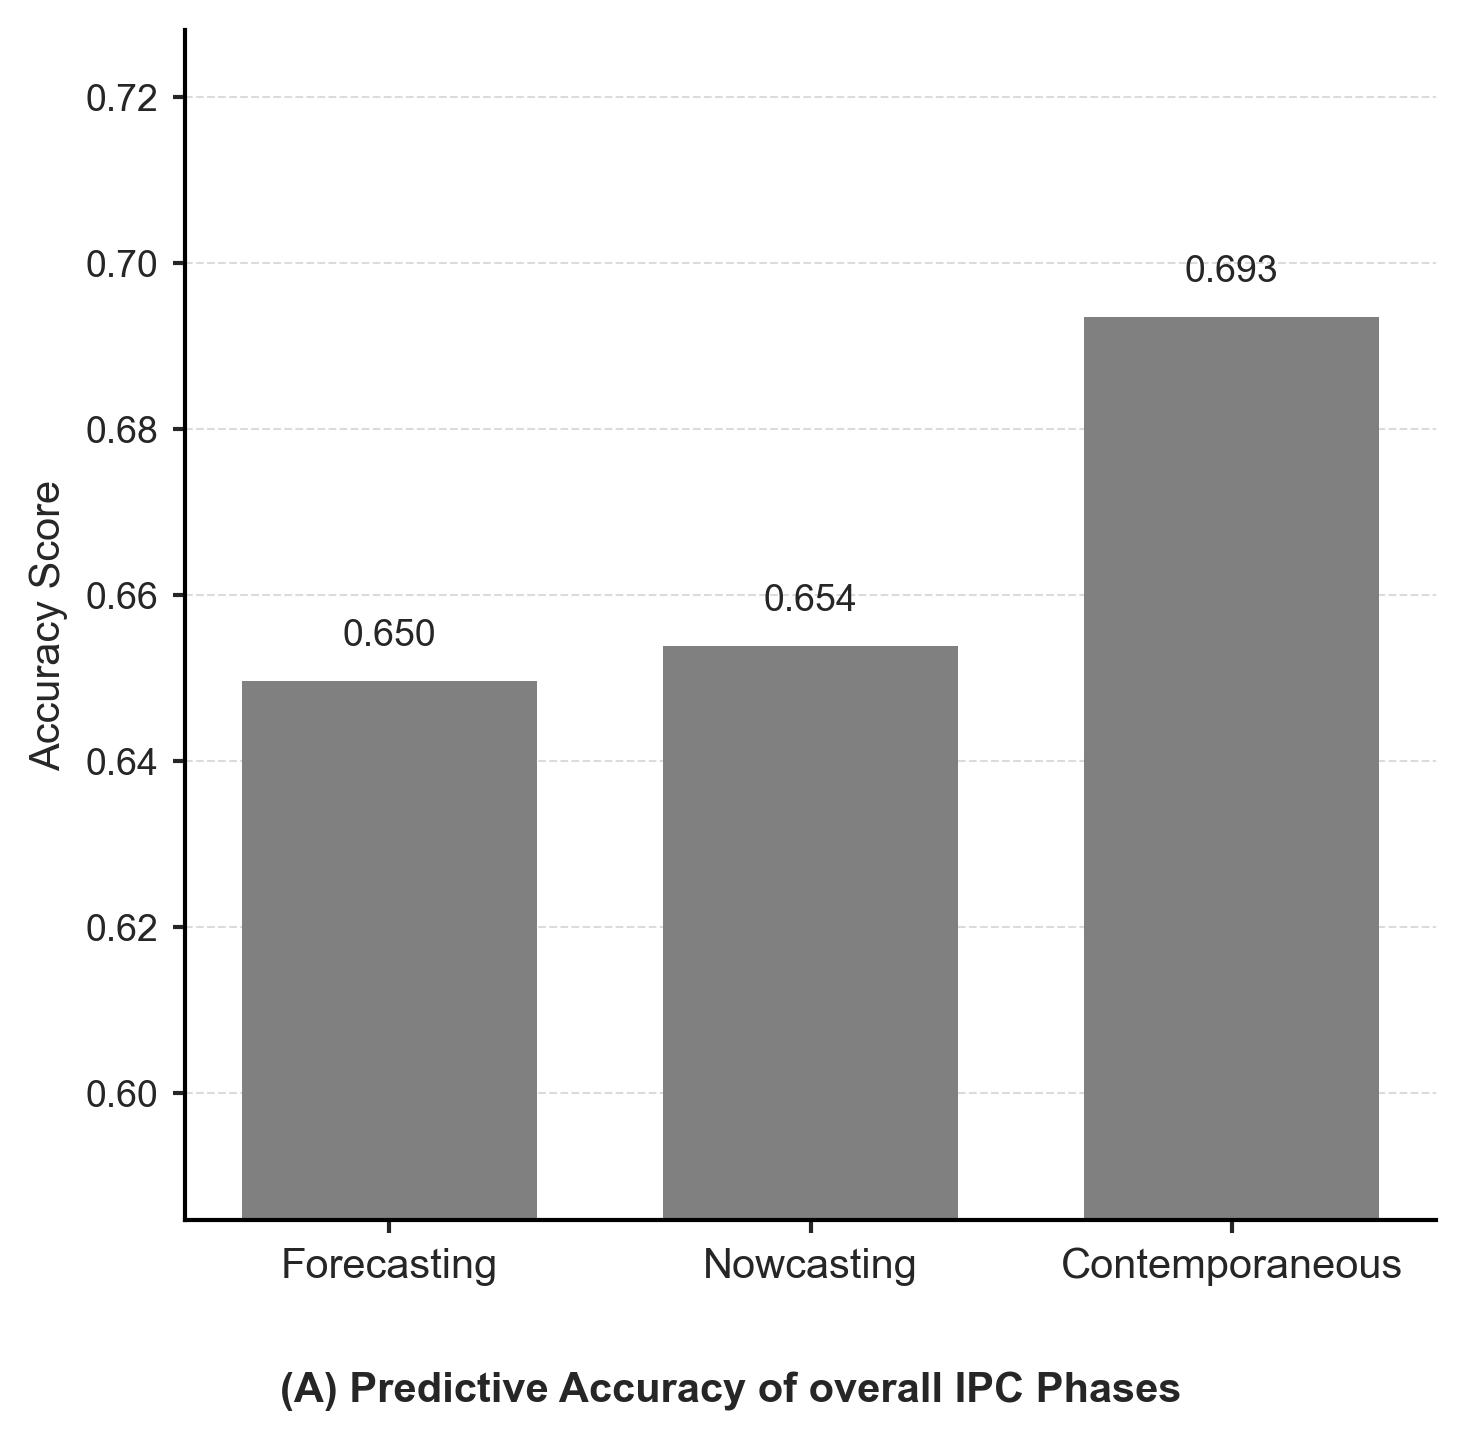
\includegraphics[width=0.40\textwidth]{accuracy.jpg} % Use ~48% of page text width
        & % Column separator
        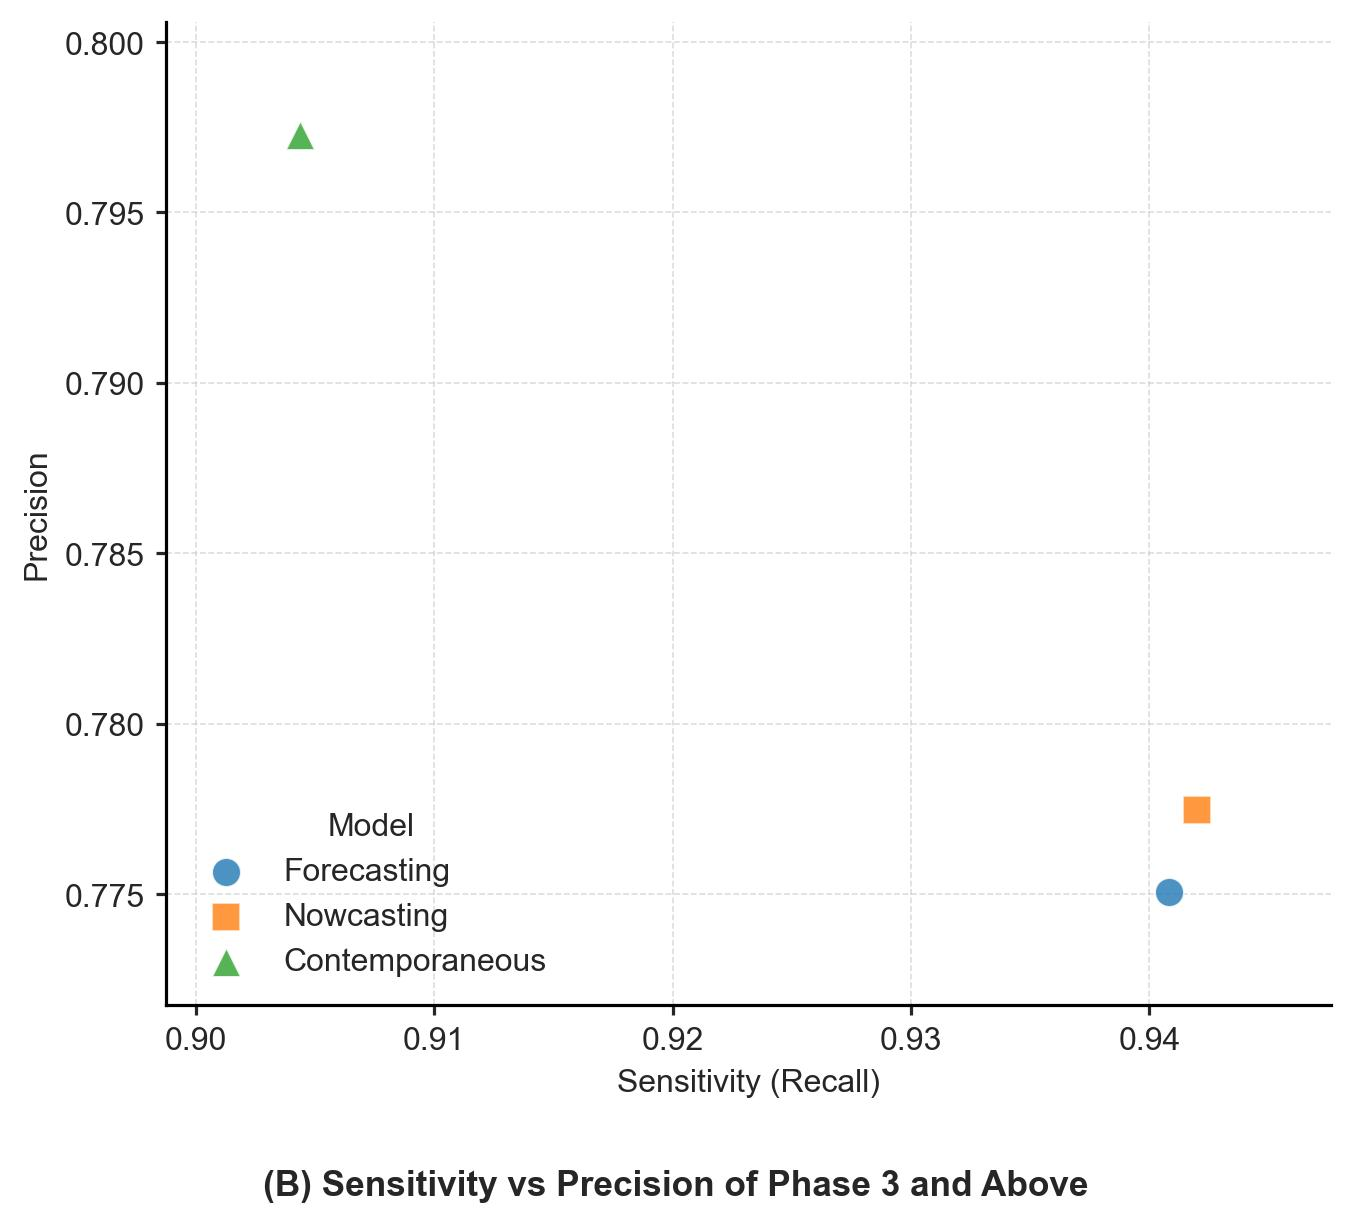
\includegraphics[width=0.40\textwidth]{precision_sensitivity.jpg} % Use ~48% of page text width
        \\ % End of Row 1

        % --- Vertical Space between rows ---
        \multicolumn{2}{c}{\vspace{0.5cm}} \\ % Keep vertical space

        % --- Row 2: Subplot 3 below, spanning columns ---
        \multicolumn{2}{c}{% Content spans 2 columns, centered 'c'
            % Make this one wider, e.g., 95% of page text width
            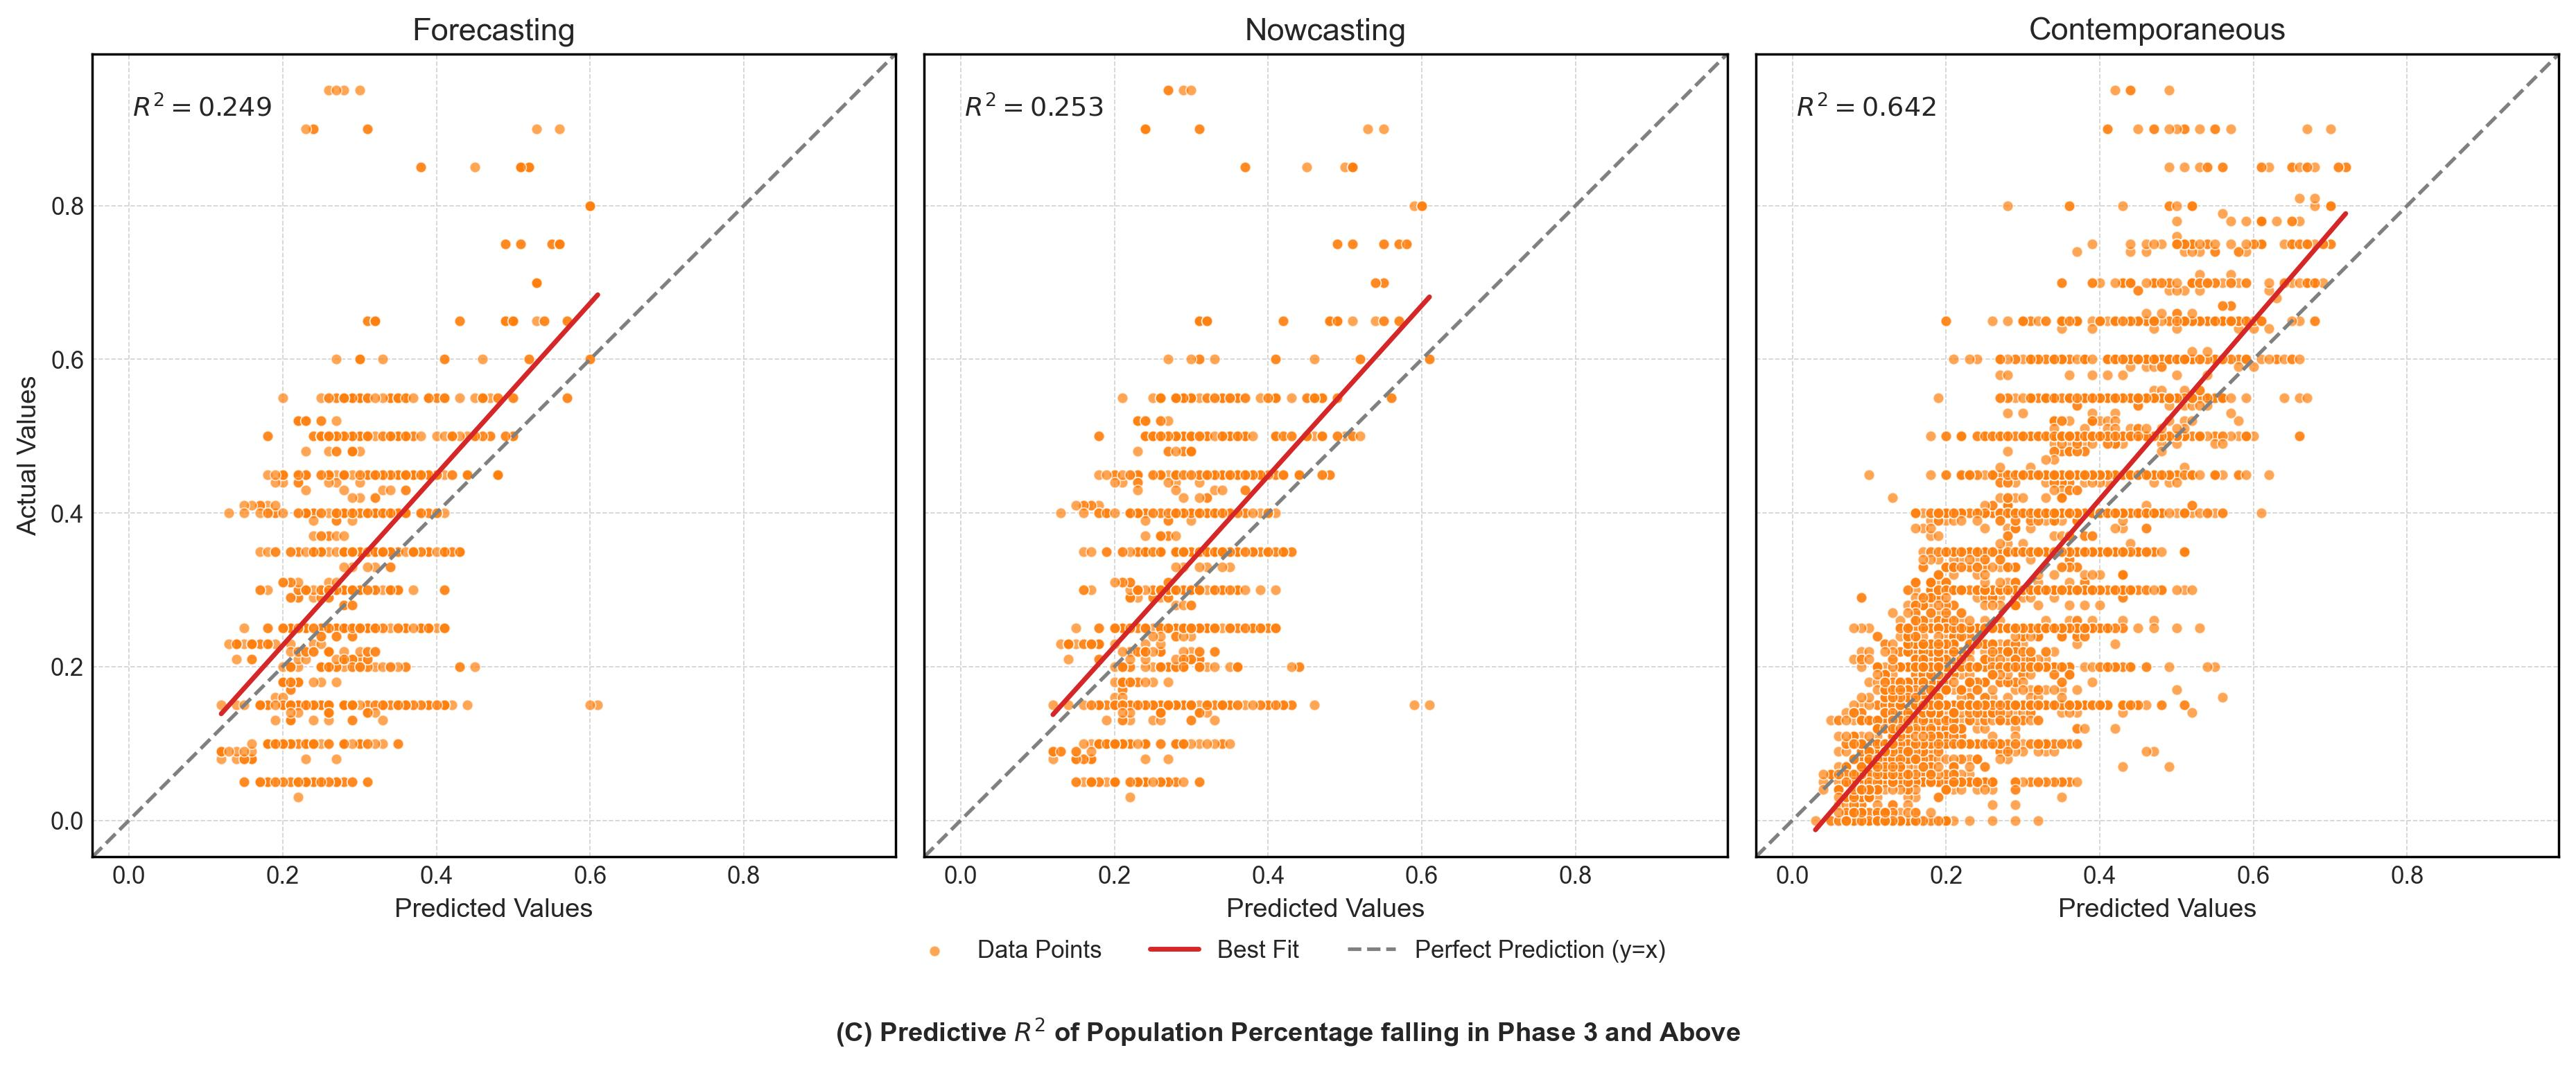
\includegraphics[width=0.95\textwidth]{R2.jpg} % Adjust 0.95 if needed
        } \\ % End of Row 2

        % --- Caption Row ---
        \multicolumn{2}{c}{\parbox{0.95\textwidth}{\centering % Add parbox for better control if needed, and centering within it
            \caption{Performance Metrics Across Forecasting, Nowcasting, and Contemporaneous Models}
            \label{fig:RF}
            % Keep label after caption (or inside caption argument)
        }} \\ % End of Caption Row

    \end{tabular}
    % \centering % This centering is now redundant for the caption itself if handled within multicolumn
    % \caption{Performance Metrics Across Forecasting, Nowcasting, and Contemporaneous Models} % MOVED
    % \label{fig:RF} % MOVED

    \begin{minipage}{0.95\textwidth}
    \footnotesize  % Smaller font for notes
    \textbf{Notes:}
        Panel A illustrates the model’s accuracy in predicting the overall IPC (Integrated Food Security Phase Classification) phase, measured as the proportion of correctly predicted phases relative to the total number of actual cases. Panel B presents the sensitivity and precision of the model’s alert classifications. An “alert” is defined as cases where the overall IPC phase is 3 or higher, signaling the need for urgent action. Sensitivity is the proportion of correctly identified alert cases out of all actual alert cases, while precision is the proportion of true alerts among all predicted alerts. Panel C displays the out-of-sample R² for the percentage of the population classified in Phase 3 or worse. It plots the predicted values against the actual observed values. In all three panels, forecasting and nowcasting use the 2022 temporal holdout ($n=1{,}170$ each), while contemporaneous results use pooled random five-fold, row-level out-of-fold predictions ($n=5{,}575$; seed 0). Evaluation populations and validation protocols therefore differ across models.
    \end{minipage}
    % This label is for the minipage/notes, consider if this is what you intend or if fig:RF is the only figure label needed.
\end{figure}


% Make sure you have these packages in your preamble
% \usepackage{graphicx}
% \usepackage{subcaption}

\newpage
\clearpage

\begin{figure}
    \centering
    \begin{tabular}{cc}
        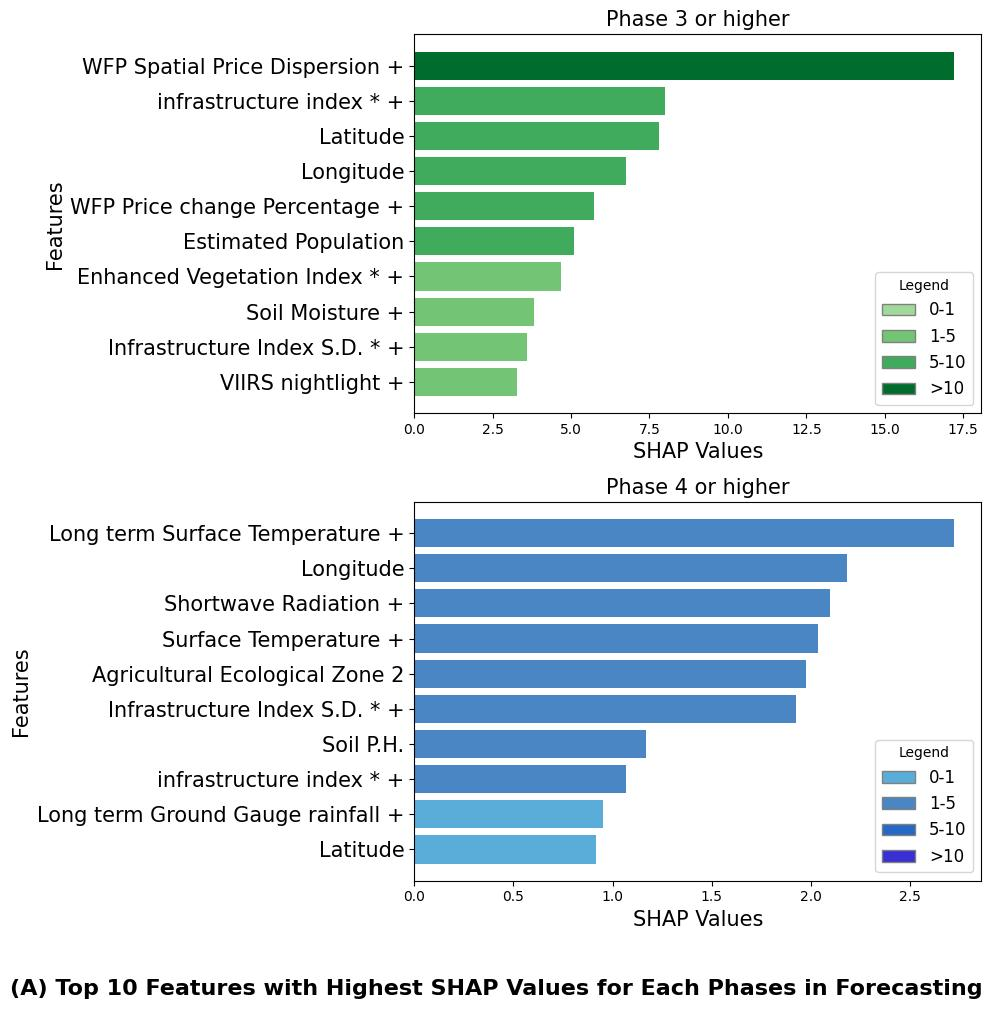
\includegraphics[width=0.43\textwidth]{Picture6.jpg} &
        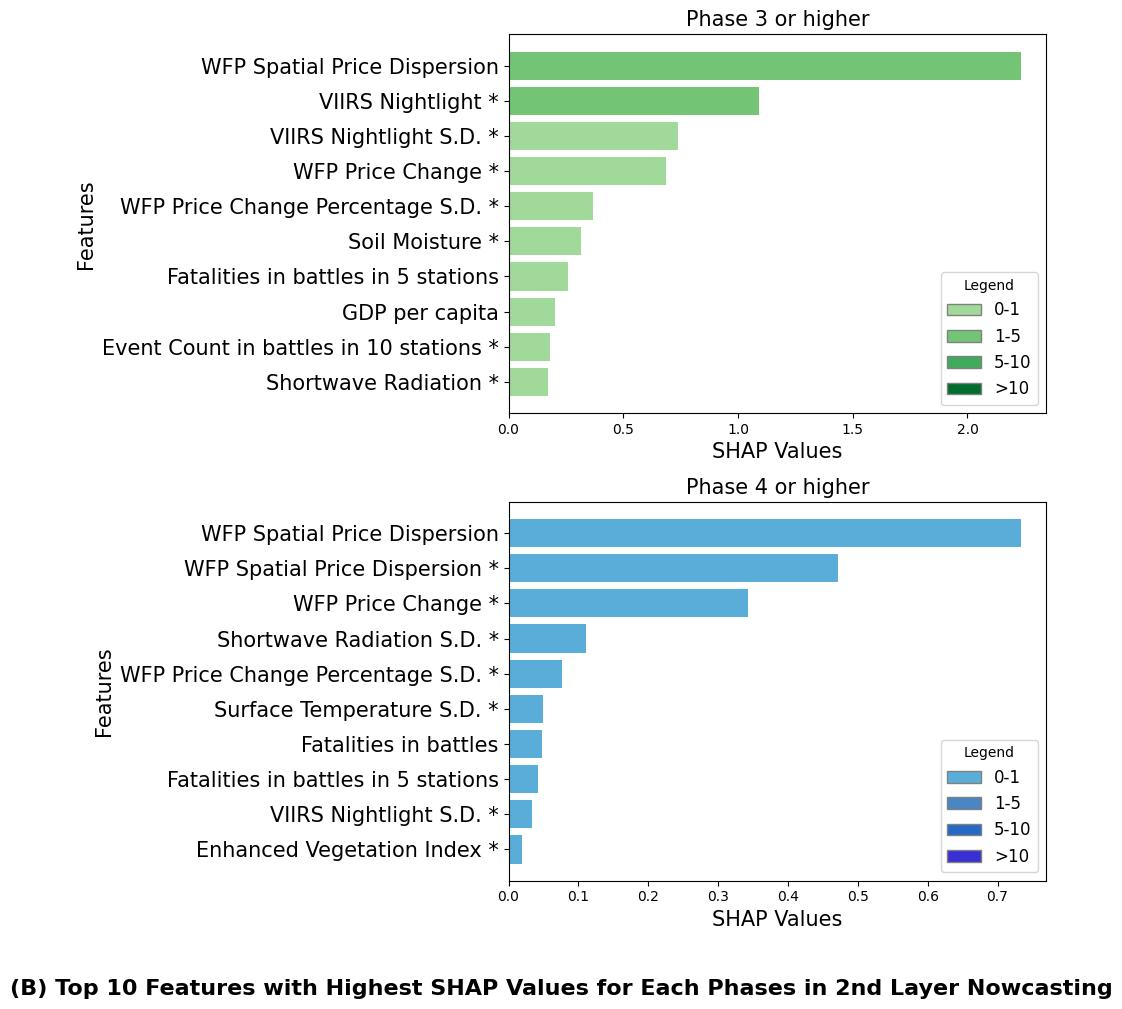
\includegraphics[width=0.48\textwidth]{Picture8.jpg} \\
        \vspace{0.5cm} & \vspace{0.5cm} \\
        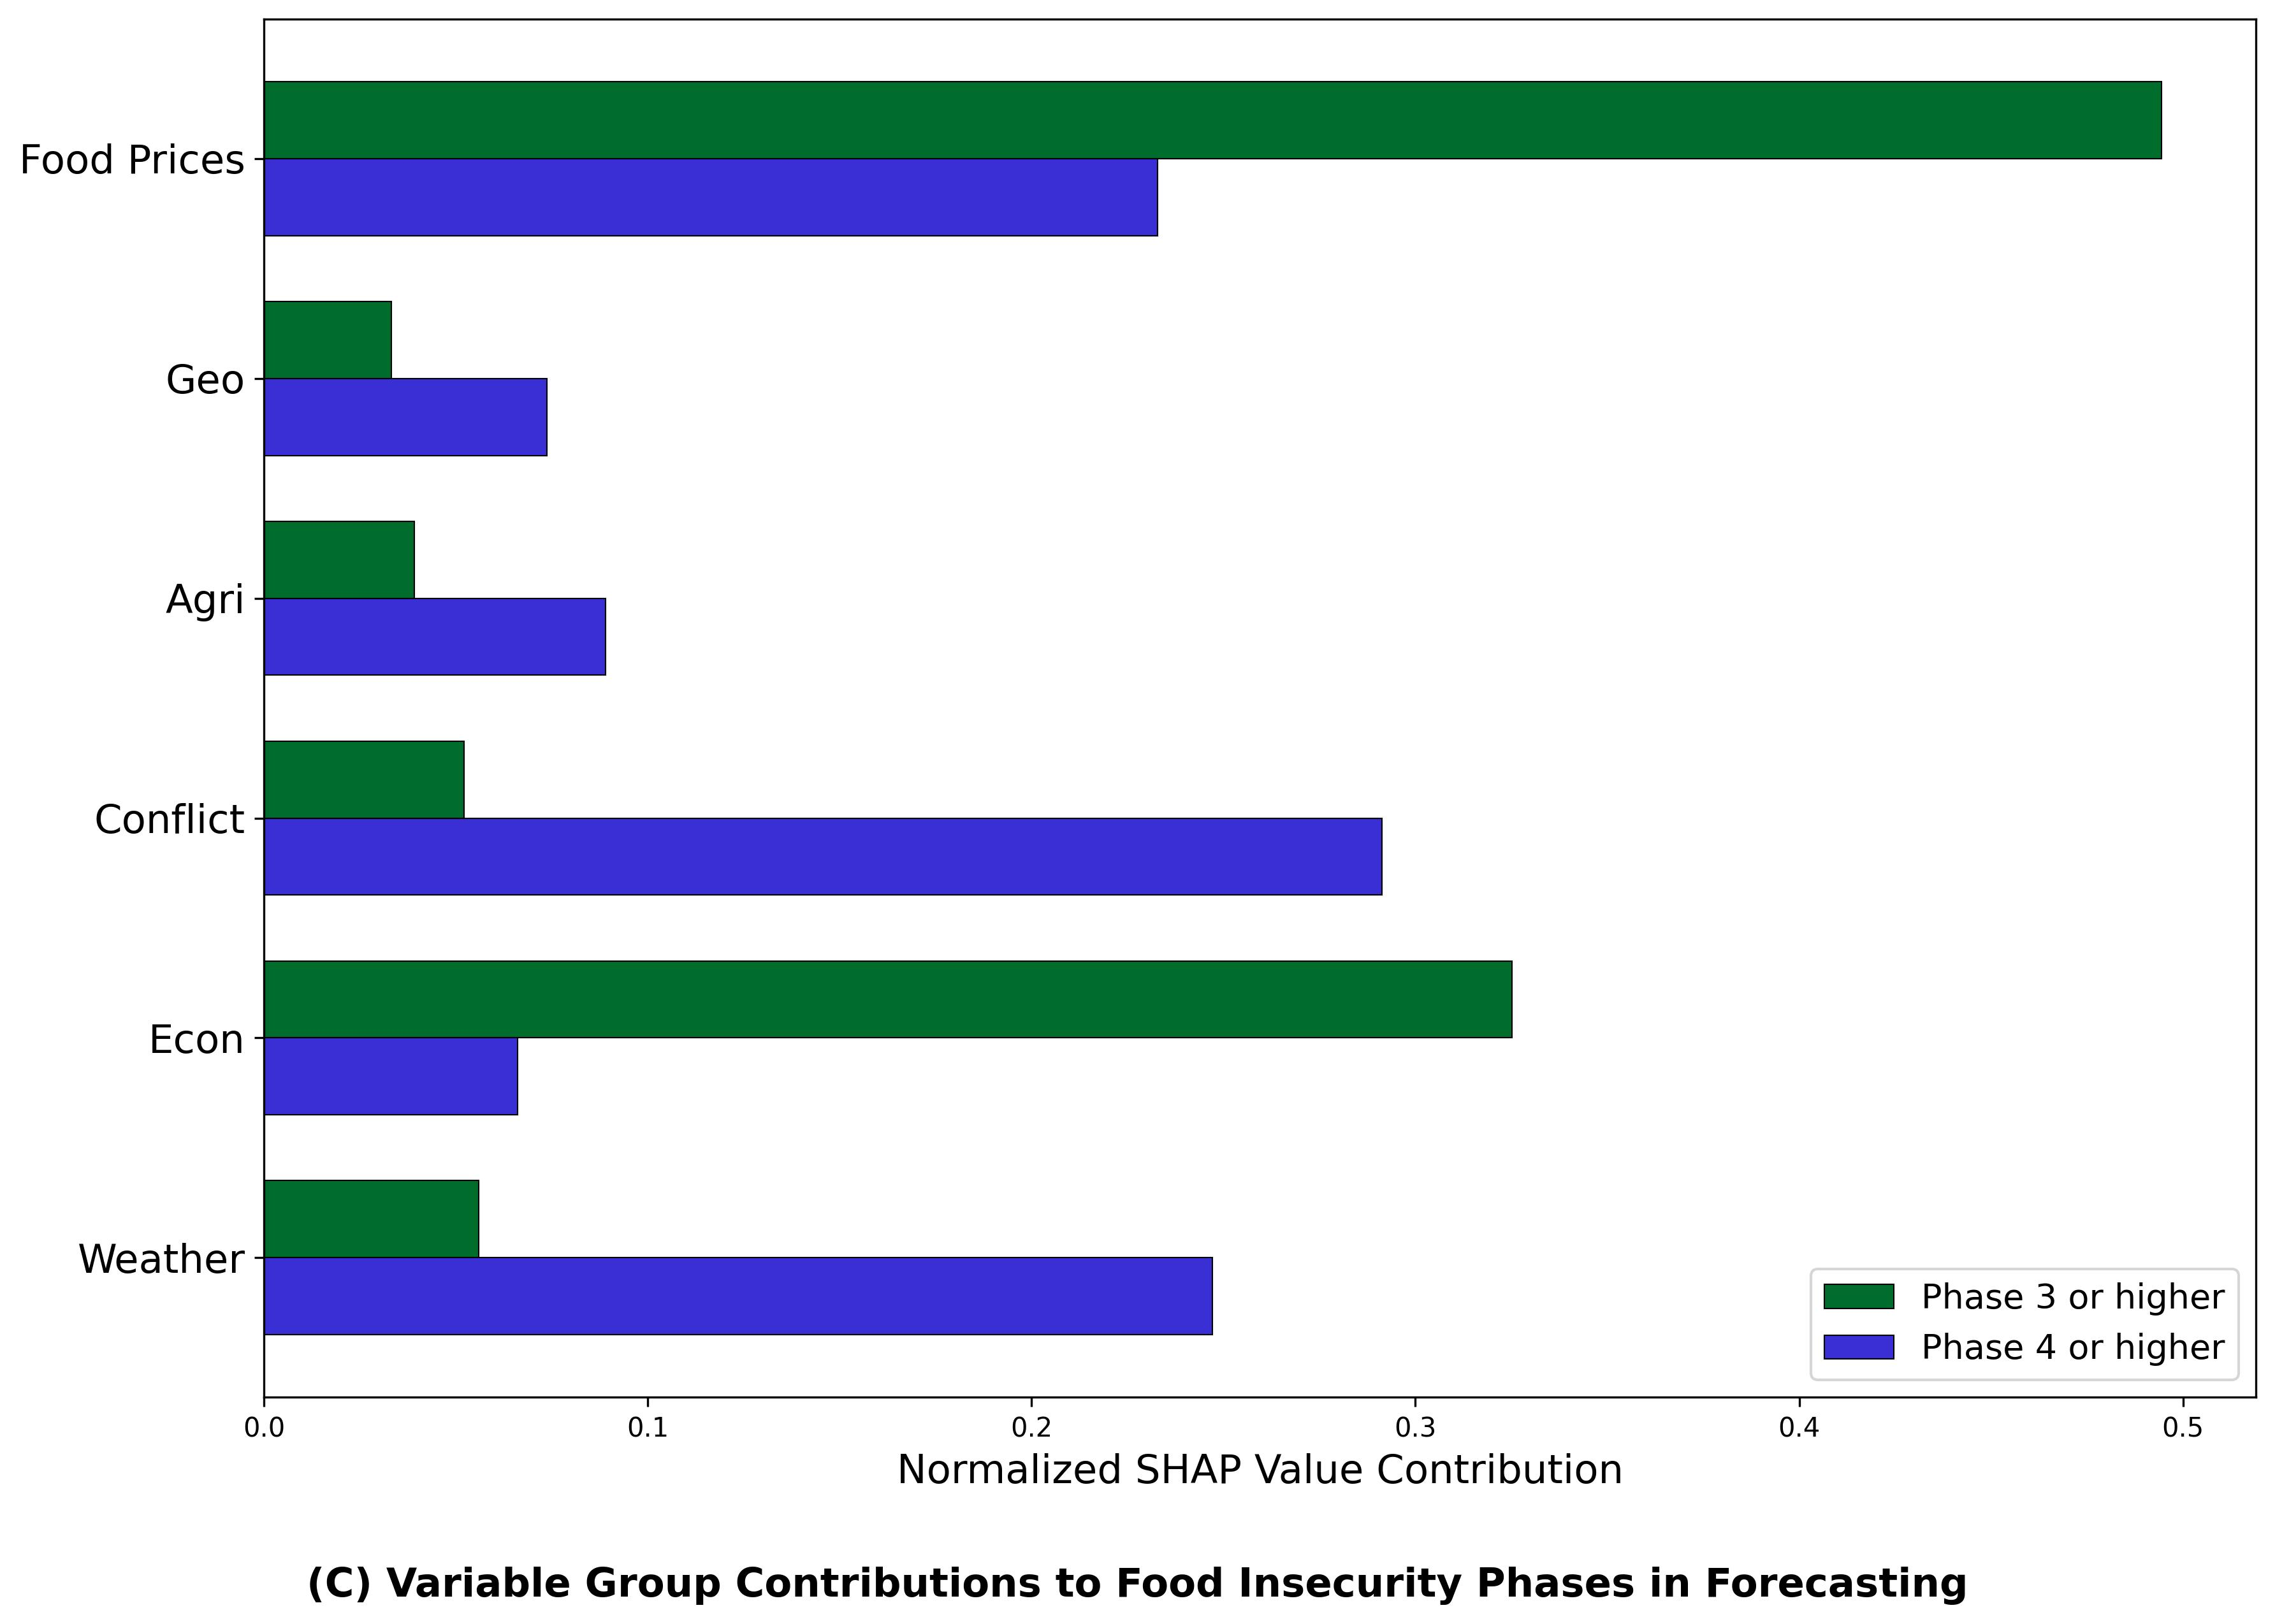
\includegraphics[width=0.47\textwidth]{Picture7.jpg} &
        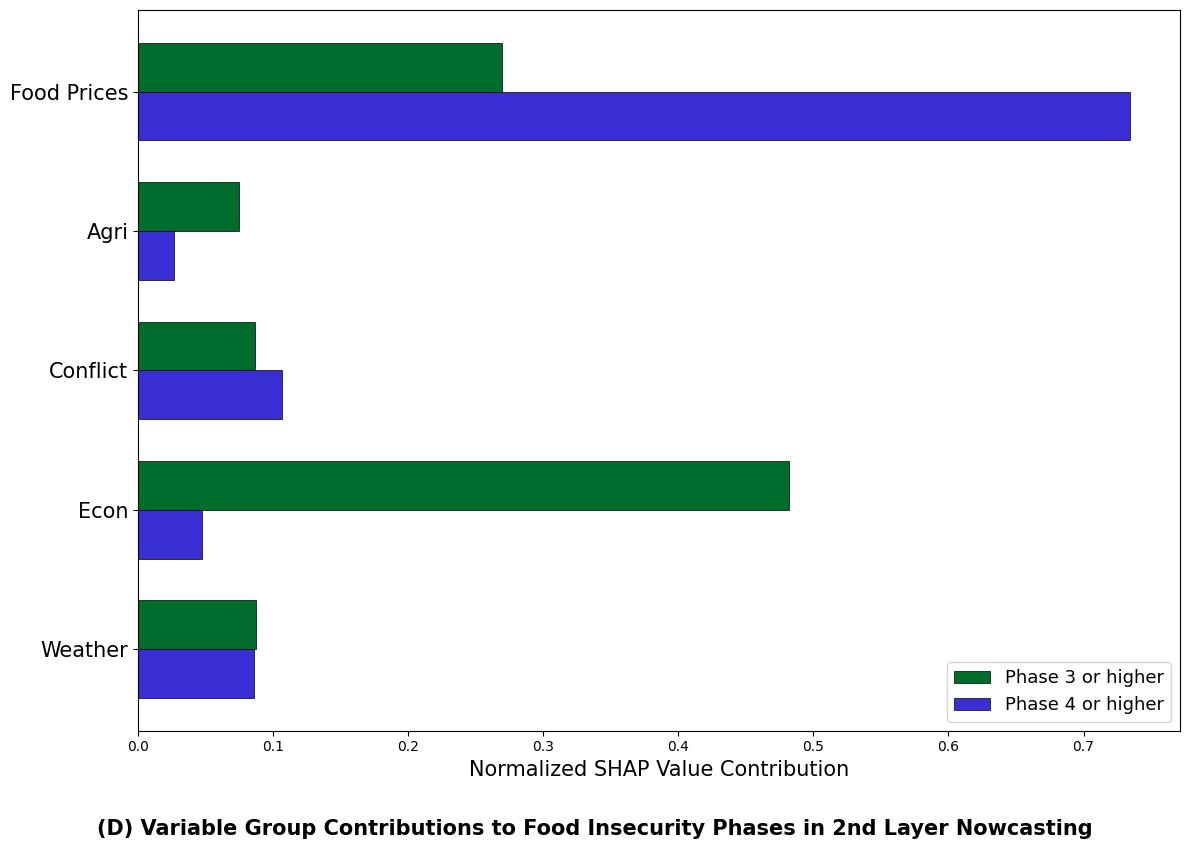
\includegraphics[width=0.47\textwidth]{Picture9.jpg} \\
         \multicolumn{2}{c}{\parbox{0.95\textwidth}{\centering % Add parbox for better control if needed, and centering within it
            \caption{Bar Chart of SHAP Value of Forecasting and Nowcasting Features}
            \label{fig:FI} % Keep label after caption (or inside caption argument)
        }} \\
    \end{tabular}
    \begin{minipage}{0.95\textwidth}
\footnotesize  % Smaller font for notes
\textbf{Notes:} 
These four panels display SHAP values, which quantify the contribution of individual variables or variable groups to food insecurity predictions. Panel A presents the SHAP values of the top individual variables in the forecasting model for Phase 3+ (top figure) and Phase 4+ (bottom figure). Panel B shows the SHAP values of the top variables in Layer 2 of the nowcasting model, again for Phase 3+ (top) and Phase 4+ (bottom). Panel C displays SHAP values aggregated by variable group in the forecasting model, with Phase 3+ results shown in green and Phase 4+ in blue. Variables are grouped into: food prices, physical geography (Geo), agriculture and land productivity (Agri), conflict, economic conditions (Econ), and weather conditions. Panel D presents the SHAP values of the same variable groups, but for Layer 2 of the nowcasting model.
In the graph, a variable name ending with “+” indicates it is lagged by 12 months, while a name ending with “\*” denotes a 12-month moving average.
\end{minipage}
\end{figure}

\newpage
\clearpage
% Preamble (once)

% Figure
\begin{figure}[htbp]
  \centering
  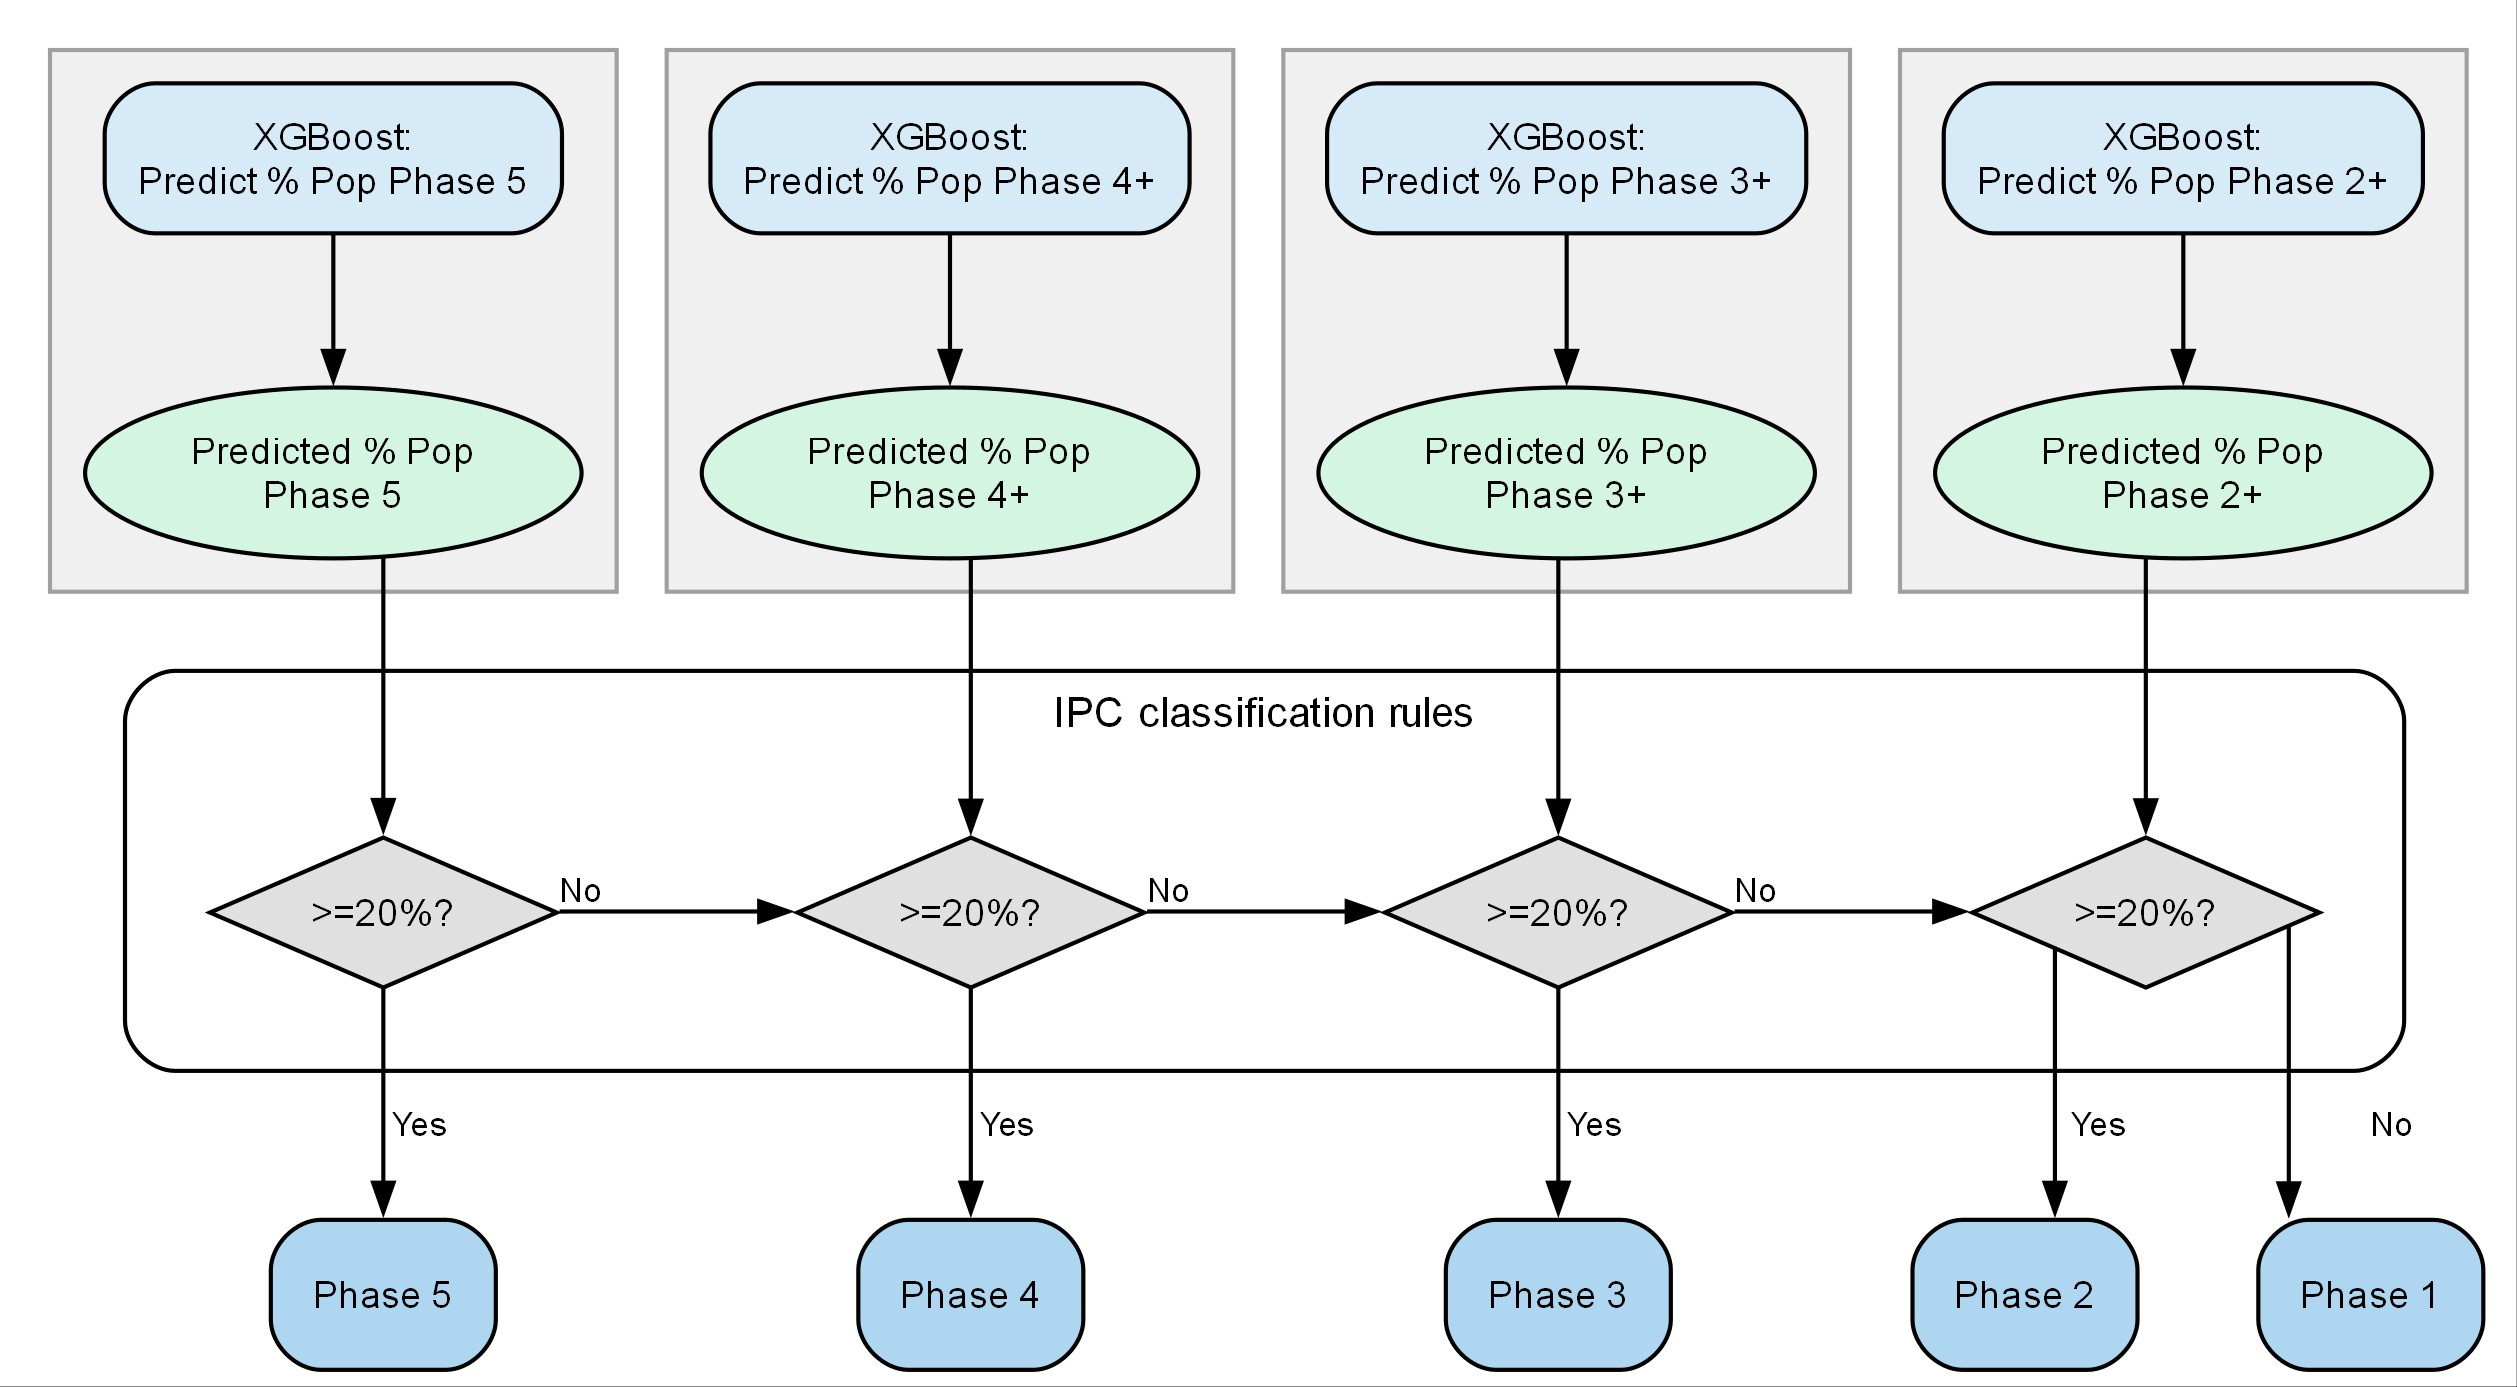
\includegraphics[width=\linewidth]{Picture3.jpg}
  \caption{Ensemble Model Procedure Overview}
  \label{fig_AP:ensemble}

  {%
    \parbox{\linewidth}{\footnotesize\raggedright
      \textbf{Notes:} This flowchart illustrates the estimation process for IPC outcome variables, namely the overall IPC phase and the percentage of the population falling into each phase. The structure follows the classification logic outlined in the FAO IPC Manual \citep{IPC2021}. We employ four separate XGBoost regression models to estimate the share of the population falling into: (i) Phase 2 or higher, (ii) Phase 3 or higher, (iii) Phase 4 or higher, and (iv) Phase 5. These outputs are combined to generate predicted population distributions across IPC phases. The overall IPC phase classification is then assigned based on a threshold rule: if at least 20\% of the population is predicted to be in Phase 5, the area is classified as IPC Phase 5; if less than 20\% is in Phase 5 but at least 20\% is in Phase 4 or higher, it is classified as Phase 4, and so on, down to Phase 1.
    }%
  }
\end{figure}


\newpage
\clearpage


% Figure
\begin{figure}[htbp]
  \centering
  % Panel A
  
\includegraphics[width=.55\linewidth]{Picture1.jpg}

  \vspace{0.8\baselineskip} % vertical gap between the two images

  % Panel B
  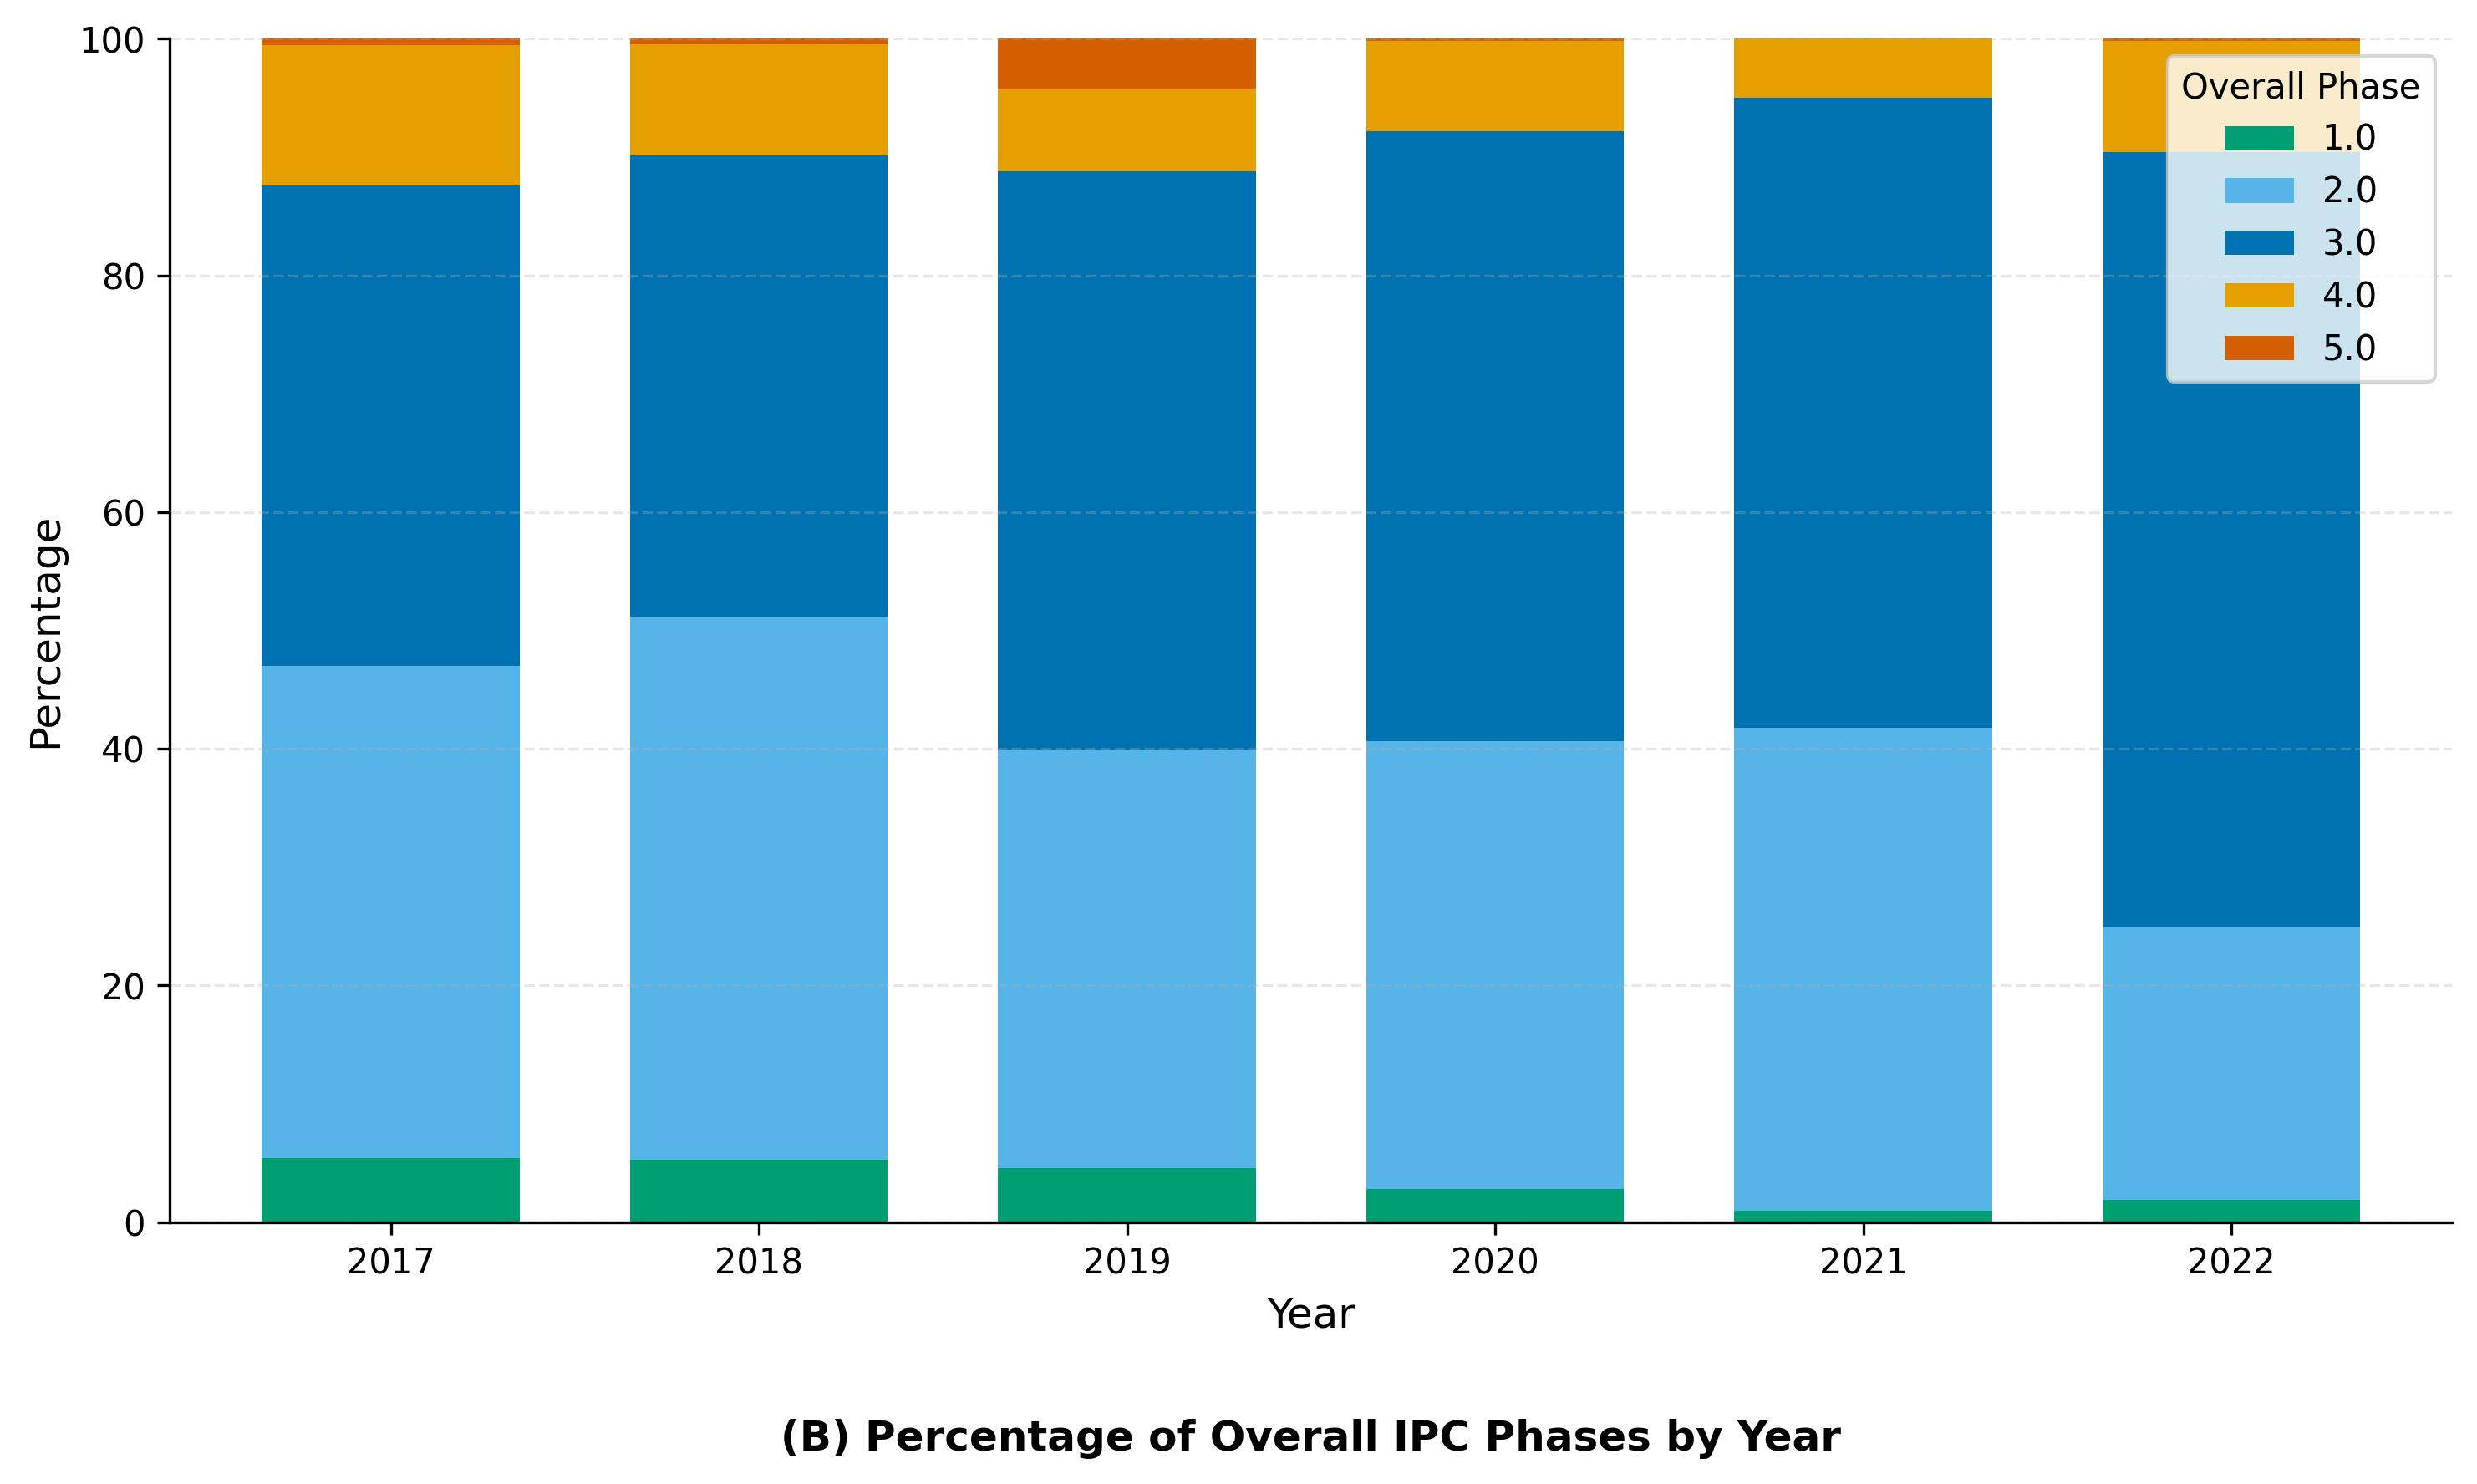
\includegraphics[width=.70\linewidth]{Picture2.jpg}

  \caption{Distribution of Overall Phase}
  \label{fig:dist}

  {%
    % Left-align ONLY the notes (main caption stays centered)
    \parbox{\linewidth}{\footnotesize\raggedright
    \textbf{Notes:}
        Panel A displays the number of instances in each IPC AFI phase from 2017 to 2022. 
      Phase 1: Minimal, Phase 2: Stressed, Phase 3: Crisis, Phase 4: Emergency, Phase 5: Famine. 
      Panel B presents the percentage distribution of cases across IPC AFI phases for each year from 2017 to 2022.
      These descriptive distributions use the overall phase labels recorded in the source data. Contemporaneous model evaluations instead use phase labels reconstructed from the observed cumulative population shares using the 20\% threshold rule; class counts can therefore differ even when the same observations are included.
    }
  }
\end{figure}



\clearpage
\newpage
\setcounter{table}{0}

\begin{table}[htbp]
\centering

\caption{Performance of Forecasting, Nowcasting, and Contemporaneous Models}
\label{tab:performance}

\begin{footnotesize}
\begin{tabular}{lcccc}
\toprule
\multicolumn{1}{c}{} & \multicolumn{4}{c}{\textbf{Performance Metrics}} \\
\cmidrule(lr){2-5}
 & \textbf{(1)} & \textbf{(2)} & \textbf{(3)} & \textbf{(4)} \\
 & \textbf{Accuracy} & \textbf{Sensitivity} & \textbf{Precision} & \textbf{R$^2$} \\
\midrule

\textbf{Panel A: Forecasting} & & & & \\
All Observations & 0.650 & 0.941 & 0.775 & 0.249 \\
Observations with Changed Phase & 0.593 & 0.990 & 0.702 & -- \\

\midrule

\textbf{Panel B: Nowcasting} & & & & \\
All Observations & 0.654 & 0.942 & 0.777 & 0.253 \\
Observations with Changed Phase & 0.571 & 0.964 & 0.733 & -- \\

\midrule

\textbf{Panel C: Contemporaneous} & & & & \\
All Observations & 0.693 & 0.904 & 0.797 & 0.642 \\

\bottomrule
\end{tabular}
\end{footnotesize}

\vspace{0.3cm}

\begin{minipage}{0.95\textwidth}
\footnotesize

\textbf{Notes:}
This table summarizes performance metrics for the forecasting, nowcasting, and contemporaneous models. Forecasting and nowcasting are trained on IPC data from 2017 to 2021 ($n=4{,}405$) and evaluated on the 2022 temporal holdout ($n=1{,}170$). Contemporaneous performance is computed from pooled random five-fold, row-level out-of-fold predictions for all 5,575 observations from 2017 to 2022 (seed 0; 4,460 training and 1,115 test observations per fold). Accuracy is defined as the proportion of correctly identified IPC phases relative to the total number of actual cases. Sensitivity and precision assess the models' ability to predict alerts, where an alert is defined as an overall IPC phase of 3 or higher, signaling the need for immediate action. Sensitivity is the proportion of true alert cases correctly identified, while precision is the proportion of true alerts among all predicted alerts. The out-of-sample R$^{2}$ value reflects the model's performance in predicting the percentage of the population classified as Phase 3 or worse.

For forecasting and nowcasting, performance is reported for two subsets of the test data: ``All Observations,'' which includes all records in the test set, and ``Observations with Changed Phases,'' which includes only those test set observations where the overall IPC phase differs from that in the most recent training set assessment. This distinction helps isolate performance in dynamically changing conditions.

\end{minipage}

\end{table}

\clearpage \newpage \setcounter{table}{0}  \setcounter{figure}{0} \setcounter{section}{0}
\renewcommand{\tablename}{Supplementary Table}
\renewcommand{\figurename}{Supplementary Fig.}
%\renewcommand{\sectionname}{Appendix Section}
%\setcounter{page}{1}
\appendix
%%%%%%%%%%%%%%%%%%%%%%%%%%%%%%%%%%%%%%%%%%%%%%%%%%%%%%%%%%%%%%%%%%%%%%%%%%%%%%%%%%%%%%%%%%%%%
\newpage
\section*{Supplementary Figures}
%\label{sec:oversample}

\begin{figure}[htbp]
  \centering
  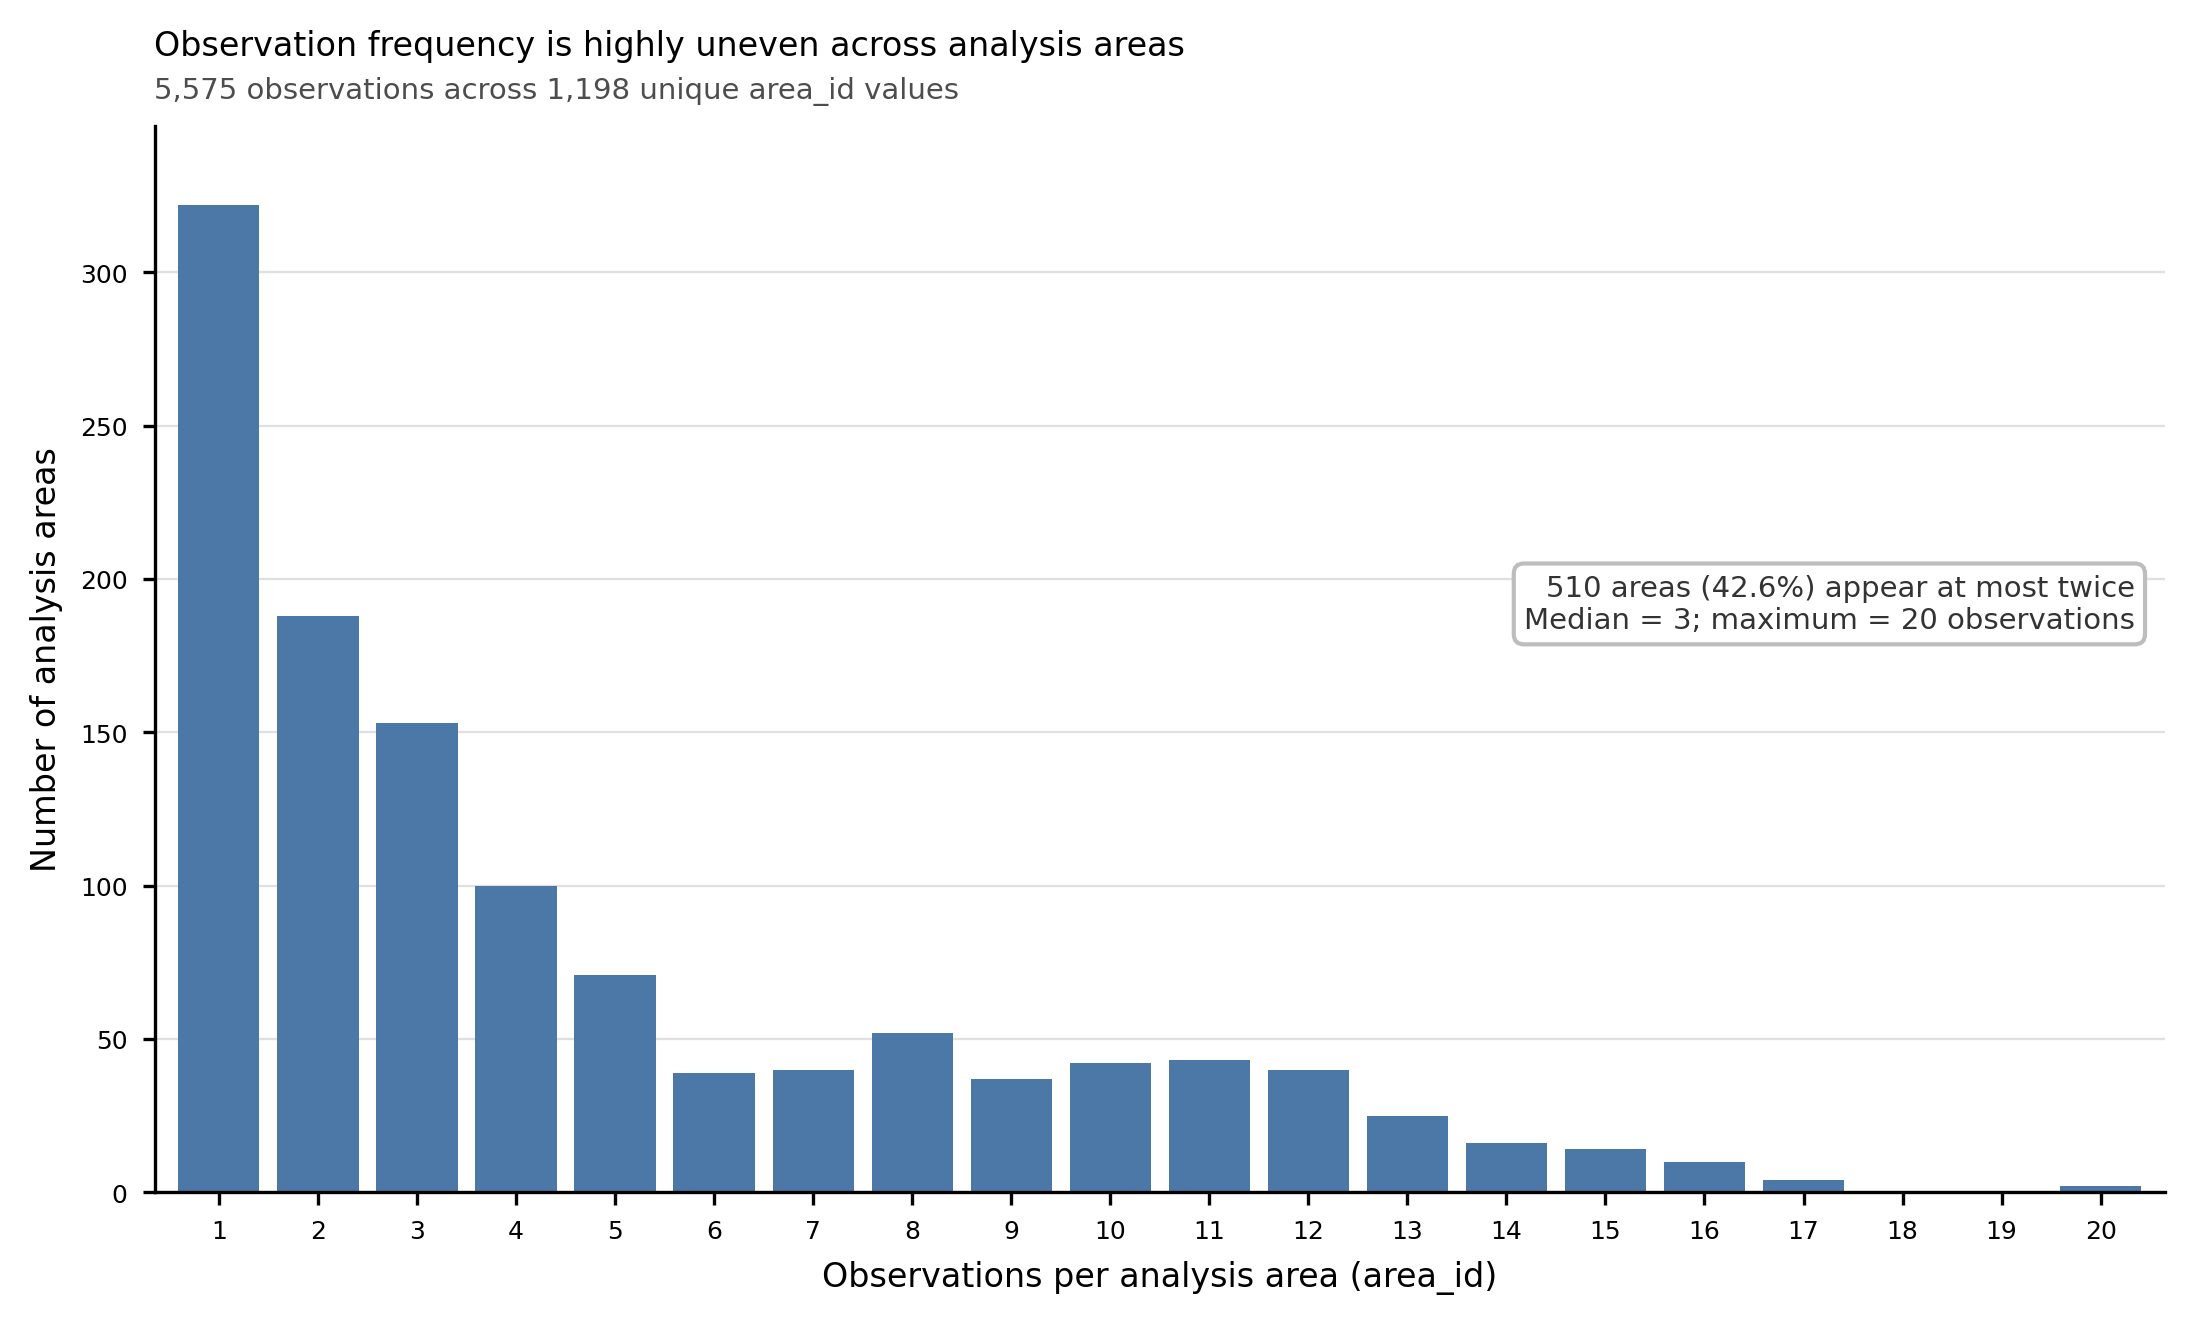
\includegraphics[width=\linewidth, height=0.8\textheight, keepaspectratio]{sample_imbalance_area_frequency.png}
  \caption{Uneven Observation Frequency Across Analysis Areas}
  \label{fig:SI_area_observation_frequency}

  \parbox{\linewidth}{\footnotesize\raggedright
    \textbf{Notes:} The histogram shows the number of observations available for each analysis area in the contemporaneous modeling sample. The horizontal axis gives the number of observations associated with an individual \texttt{area\_id}, and the vertical axis gives the number of unique analysis areas with that observation frequency. The sample contains 5,575 observations from 1,198 unique analysis areas. Observation frequency is strongly unbalanced: 510 areas (42.6\%) appear no more than twice, the median area appears three times, and the maximum number of observations for a single area is 20. This imbalance motivates reporting row-level cross-validation results separately from validation designs that explicitly account for repeated observations or geographic grouping.
  }
\end{figure}

\newpage
\begin{figure}[htbp]
  \centering
  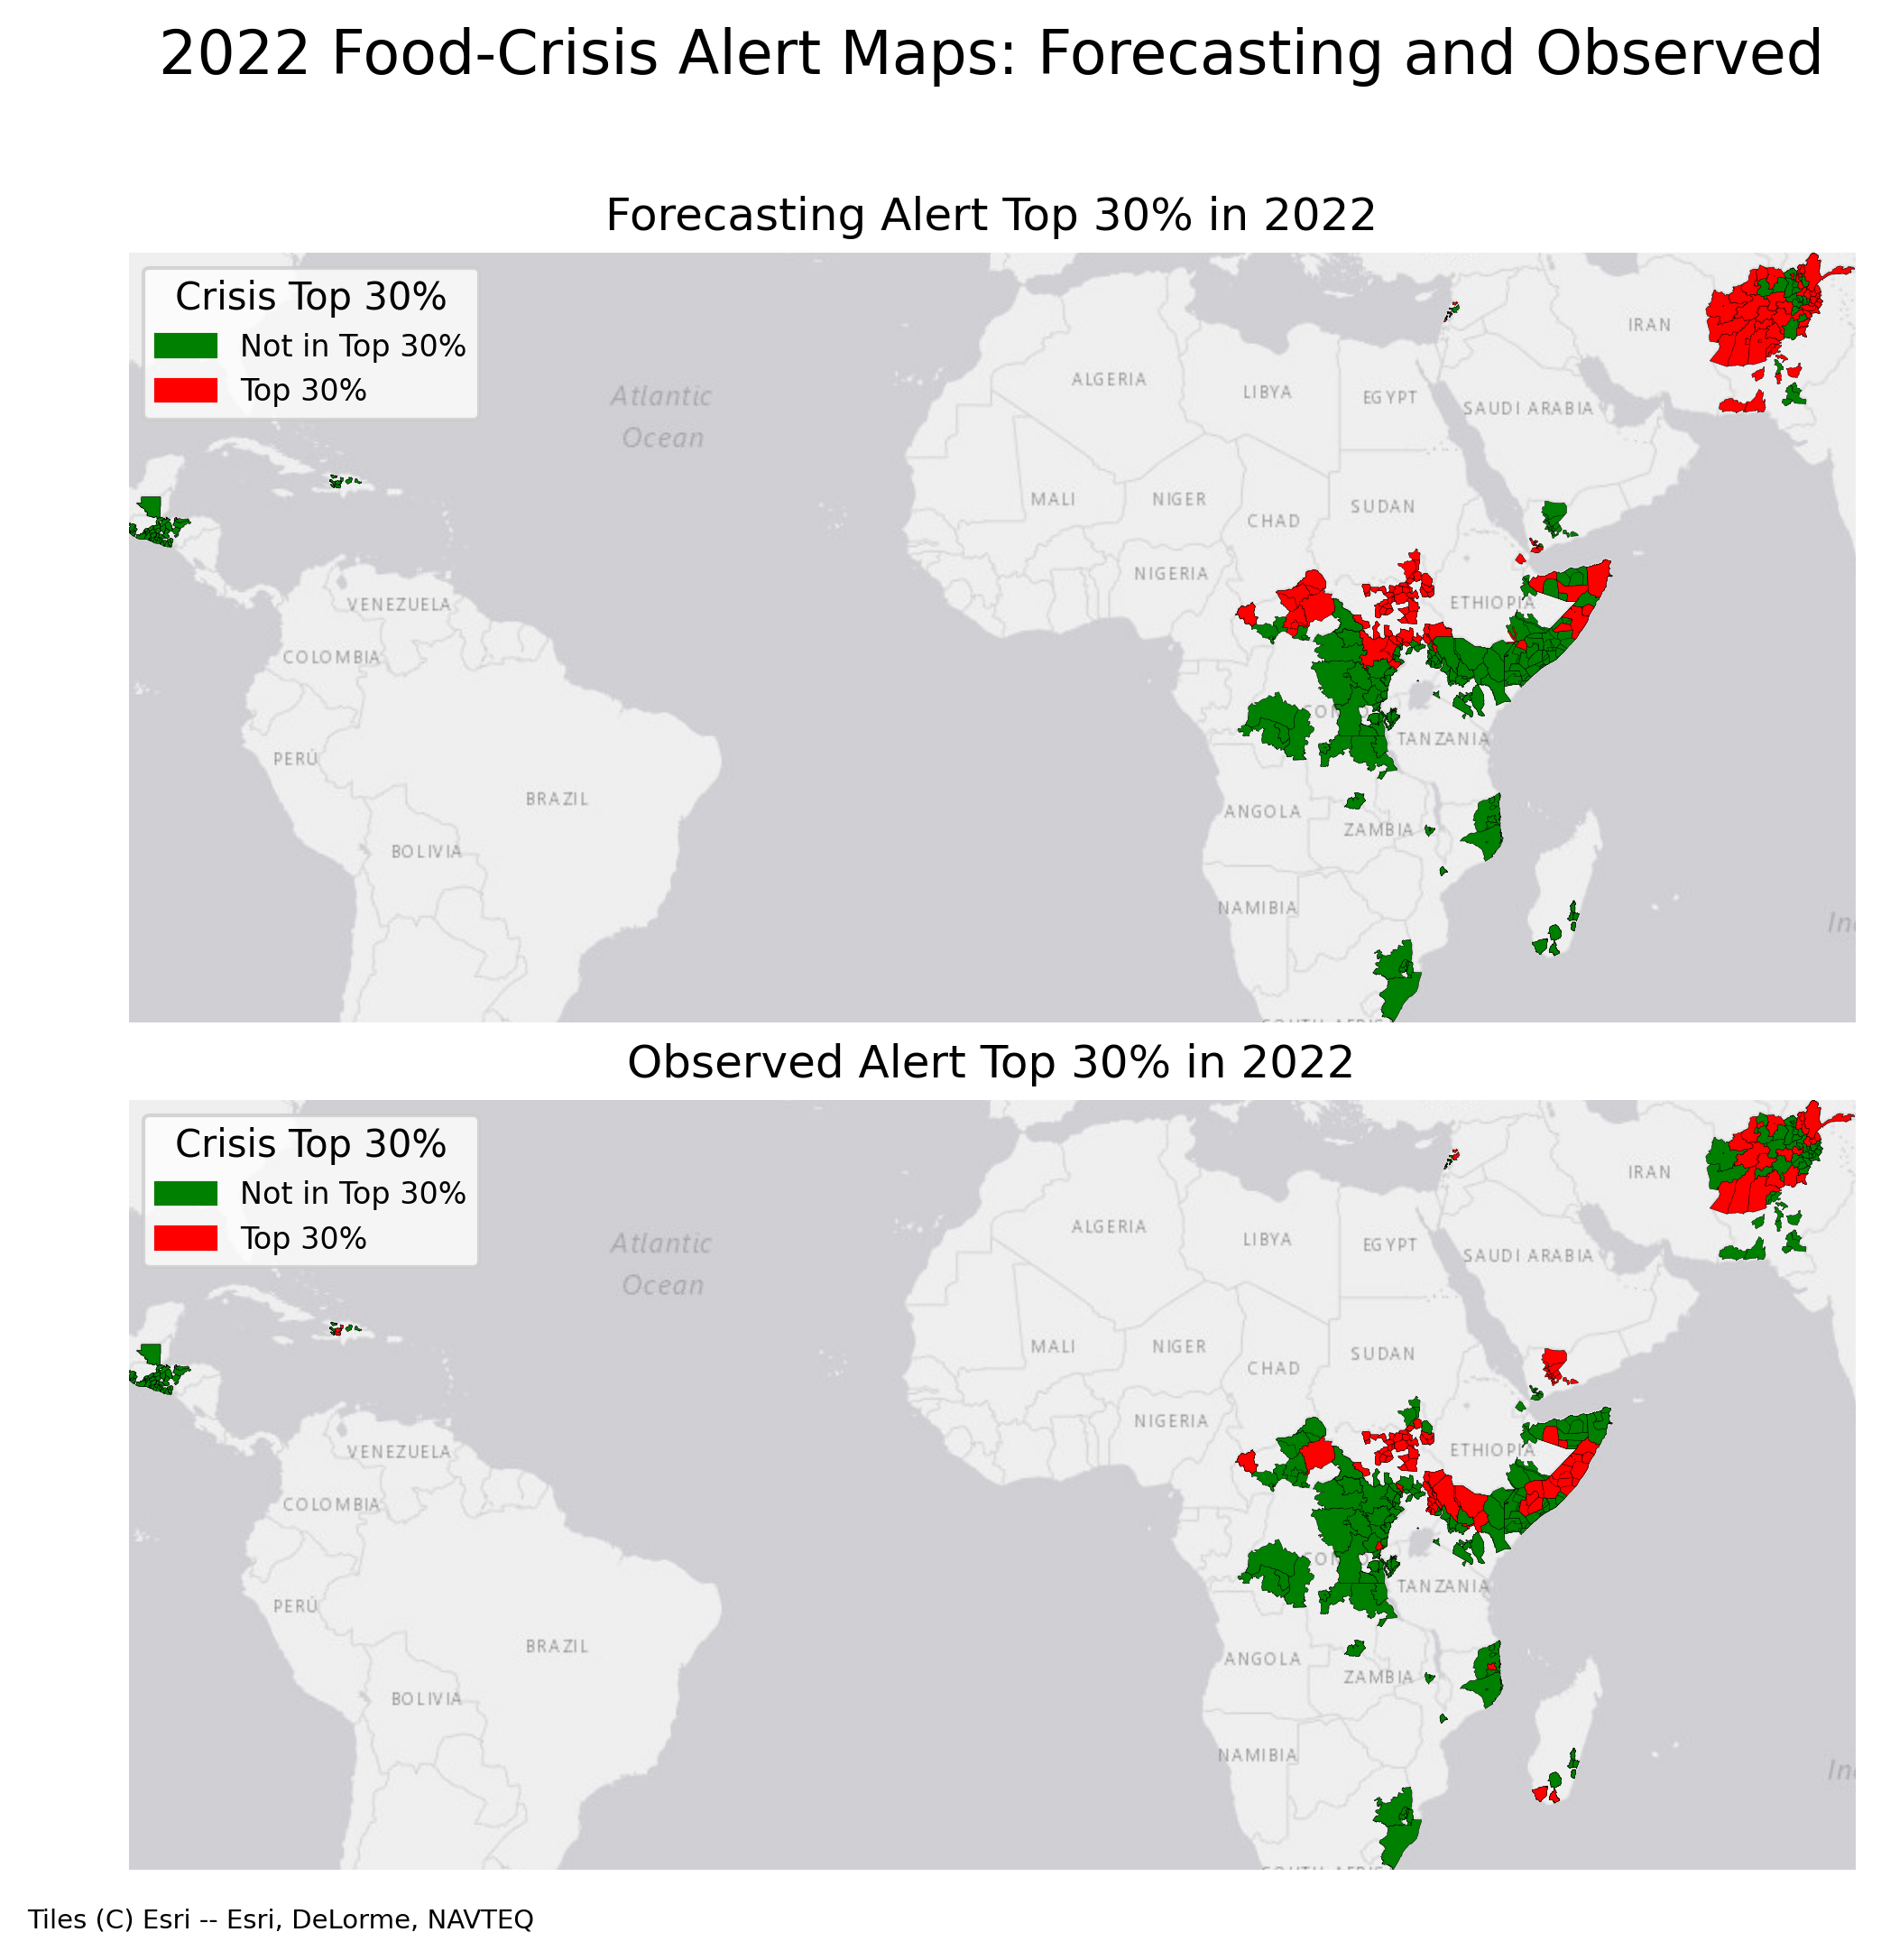
\includegraphics[width=\linewidth, height=0.8\textheight, keepaspectratio]{2022_alert_map_panel_2x3.png}
  \caption{Top 30\% Predicted and Observed Food-Insecure Areas by Population Share in Food Crisis}
  \label{fig:SI_2022_alert_maps}

  \parbox{\linewidth}{\footnotesize\raggedright
    \textbf{Notes:} The maps compare the spatial distribution of analysis areas in the highest 30\% of the population share experiencing food crisis. Red areas in the upper panel indicate locations predicted, 12 months in advance, to fall within the top 30\%, while red areas in the lower panel indicate locations in the top 30\% based on observed outcomes. The remaining evaluated areas are shown in green. Using the same threshold facilitates comparison of the geographic concentration and correspondence between predicted and observed high-risk areas. Gray background regions and place labels are provided only for geographic reference and do not indicate the availability of evaluation observations.
  }
\end{figure}

\newpage
\begin{figure}[htbp]
  \centering
  
\includegraphics[width=\linewidth, height=0.8\textheight, keepaspectratio]{Picture4.jpg}
  \caption{Temporal Validation for Forecasting Hyperparameter Selection}
  \label{fig_AP:tuning}
  \parbox{\linewidth}{\footnotesize\raggedright
    \textbf{Notes:} Forecasting hyperparameters were selected using four expanding-window temporal validation folds restricted to 2017–2021, adapted from \citep{westerveld2021forecasting}. Training began with 2017, followed by validation in 2018; subsequent folds expanded training annually and validated in 2019, 2020 and 2021. The 2022 observations were excluded from every tuning fold. For final forecasting and nowcasting evaluation, observations from 2017–2021 formed the training set and 2022 observations formed the fixed held-out test set. Nowcasting and contemporaneous models were evaluated with fixed hyperparameters, without separate hyperparameter searches.
  }
\end{figure}


\begin{figure}[htbp]
  \centering
  
\includegraphics[width=\linewidth, height=0.8\textheight, keepaspectratio]{direct_phase3_vs_phase45_rescue_five_class_confusion_atlas.png}
  \caption{IPC Predictions Before and After Combined Phase 4/5 Rescue}
  \label{fig:SI_five_class_rescue_confusion}

  \parbox{\linewidth}{\footnotesize\raggedright
    \textbf{Notes:} For the contemporaneous panels, actual phases are reconstructed from the observed cumulative population shares using the model's 20\% threshold rule, rather than taken from the source-table phase labels used in Fig.~\ref{fig:dist}.
    Rows show forecasting (a--b), nowcasting (c--d), and contemporaneous modeling (e--f). Left panels retain five predicted IPC classes. Right panels display four predicted categories (P1, P2, P3, combined P4/5), summing the stored P4 and P5 columns. Both sides retain all five actual classes and identical observations. Rescue promotes eligible baseline P3 predictions to combined P4/5; it does not distinguish P4 from P5 or establish improved full five-class classification. Cells report counts and percentages within each actual phase; shading represents the same within-class share. Forecasting and nowcasting use the square-root-balance policy on the 2022 temporal holdout ($n=1{,}170$ each). Contemporaneous uses the full-balance policy and seed-0 random five-fold row-level OOF predictions ($n=5{,}575$), with its threshold selected from pooled OOF results. Protocols and populations differ across rows, so cross-row performance is not directly comparable.  }
\end{figure}


\begin{figure}[htbp]
  \centering
  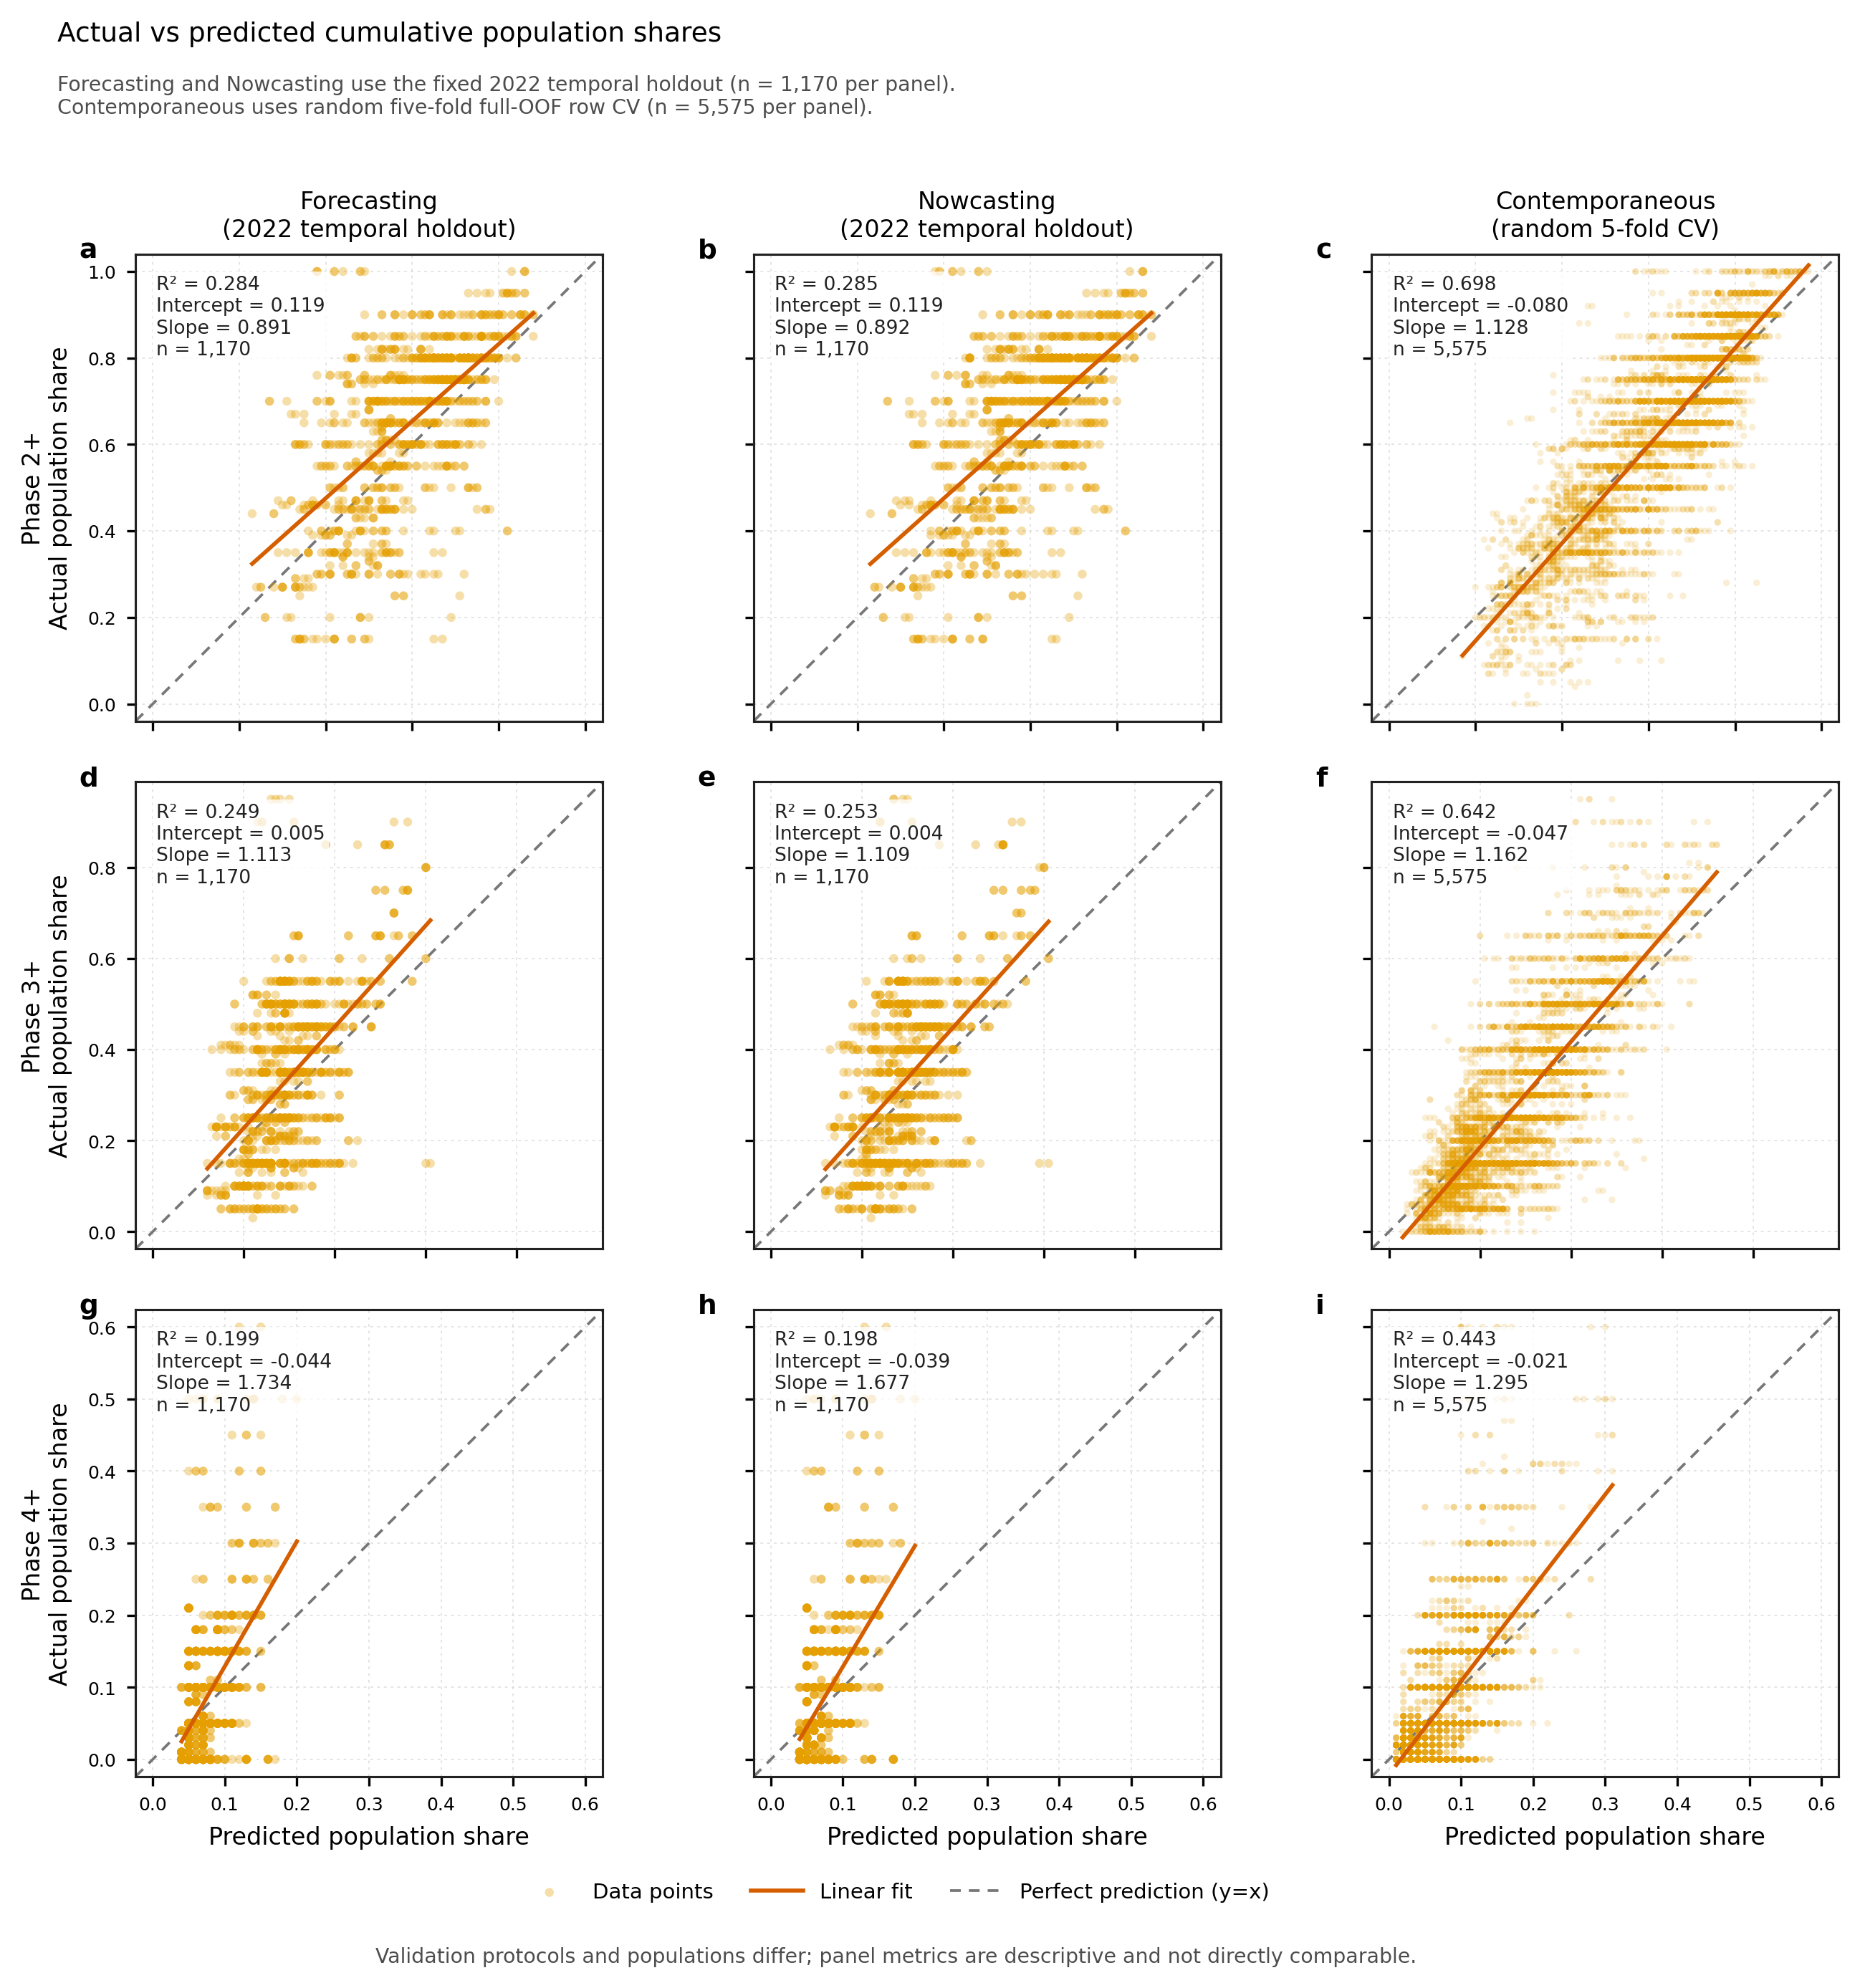
\includegraphics[width=\linewidth, height=0.8\textheight, keepaspectratio]{phase_cumulative_actual_vs_predicted_forecasting_nowcasting_contemporaneous.png}
  \caption{Actual and Predicted Cumulative IPC Population Shares}
  \label{fig:SI_cumulative_phase_shares}

  \parbox{\linewidth}{\footnotesize\raggedright
    \textbf{Notes:} These diagnostics assess cumulative population-share predictions, not probabilities that an area experiences a food crisis. Columns show forecasting, nowcasting, and contemporaneous estimates. Rows show IPC Phase 2+ (panels a--c), Phase 3+ (panels d--f), and Phase 4+ (panels g--i). Each point represents one observation, with predicted share on the horizontal axis and observed share on the vertical axis. Orange lines regress observed shares on predicted shares; dashed gray lines show equality ($y=x$). Intercept 0 and slope 1 are the linear-calibration reference. Reported $R^2$ compares the original share predictions with observations, rather than measuring the orange line's fit. Forecasting and nowcasting use the 2022 temporal holdout ($n=1{,}170$ per panel); contemporaneous estimates use random five-fold OOF predictions ($n=5{,}575$ per panel). Statistics are descriptive and not directly comparable across columns because evaluation protocols and populations differ.
  }
\end{figure}

\begin{figure}[htbp]
  \centering
  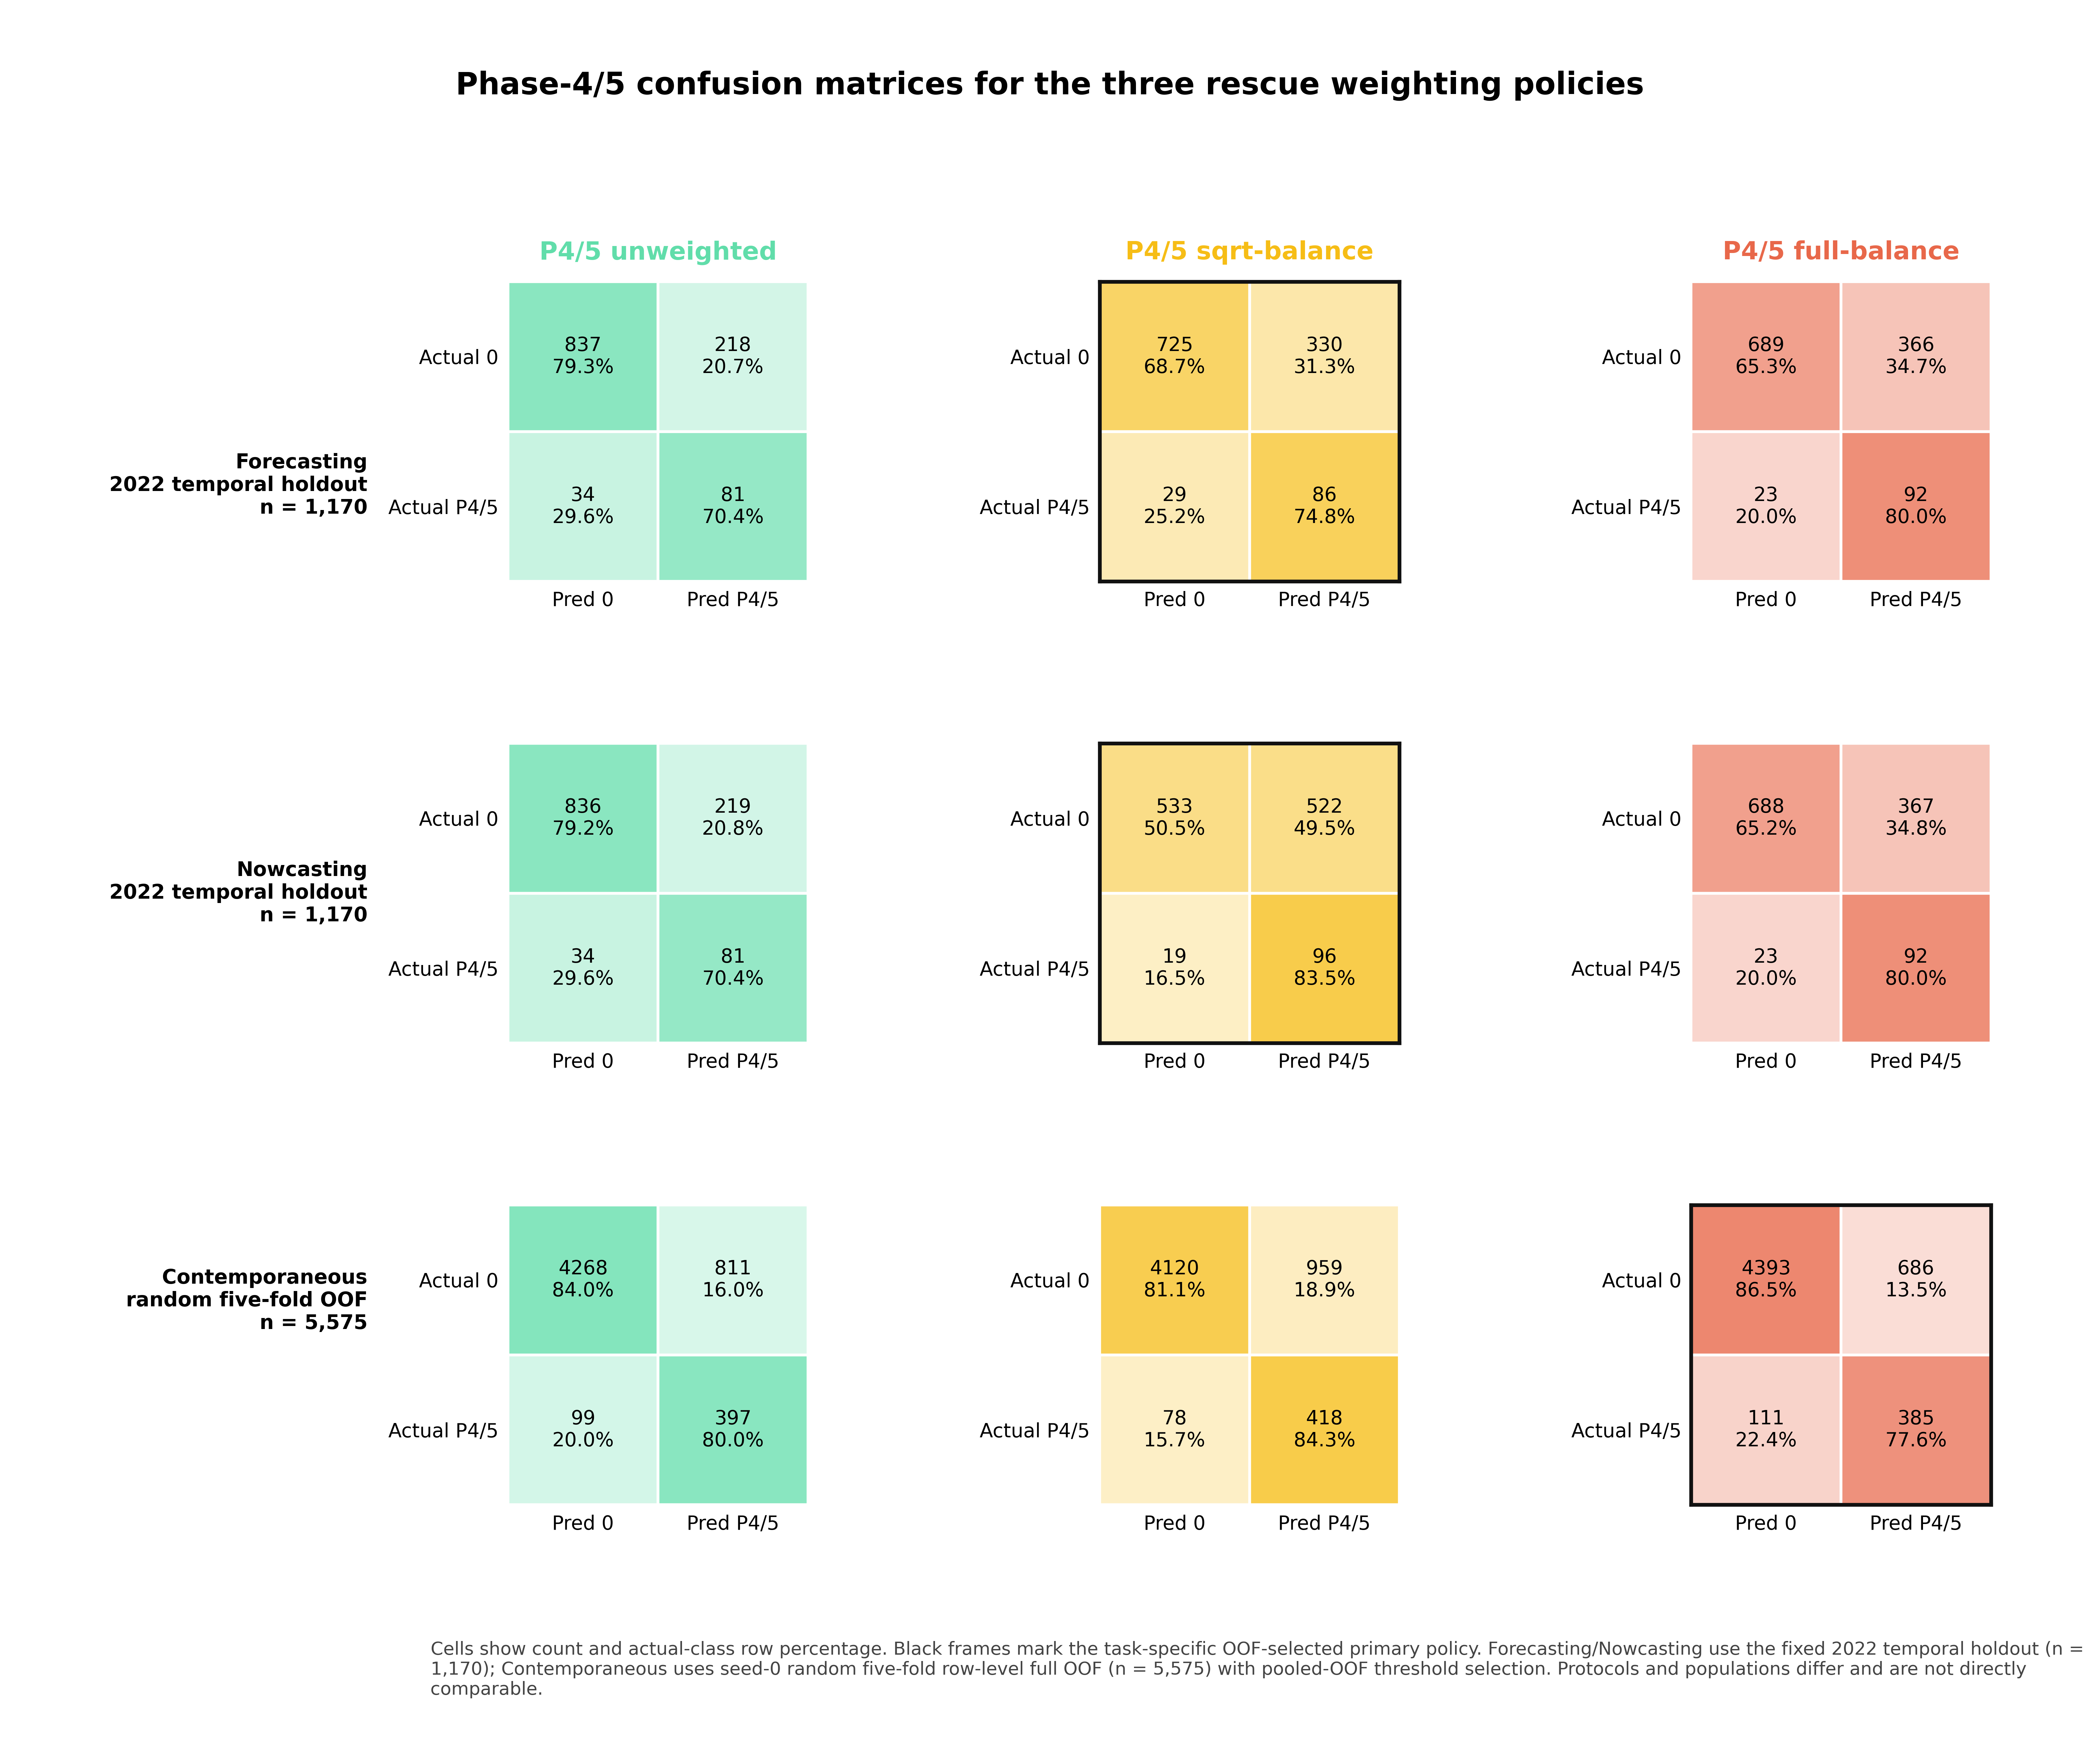
\includegraphics[width=\linewidth, height=0.8\textheight, keepaspectratio]{direct_phase3_vs_phase45_rescue_binary_confusion_atlas.png}
  \caption{Binary Confusion Matrices for the Phase 4/5 Rescue Models}
  \label{fig:SI_binary_rescue_confusion}

  \parbox{\linewidth}{\footnotesize\raggedright
    \textbf{Notes:} The matrices summarize binary classification performance for identifying observations in IPC Phase 4 or 5 under three class-weighting policies: unweighted, square-root balance, and full balance. Rows correspond to forecasting, nowcasting, and contemporaneous models, while columns correspond to the three weighting policies. ``Actual 0'' denotes observations below Phase 4, and ``Actual P4/5'' denotes observations in Phase 4 or 5. Each cell reports the observation count and the percentage within the corresponding actual-class row. Black borders identify the primary policy selected separately for each modeling task using out-of-fold (OOF) results. Forecasting and nowcasting are evaluated on the fixed 2022 temporal holdout ($n=1{,}170$ each), whereas the contemporaneous model uses seeded random five-fold, row-level OOF predictions ($n=5{,}575$), with its threshold selected from the pooled OOF predictions. Because the validation protocols and evaluation populations differ, performance should not be compared directly across modeling tasks.
  }
\end{figure}


\clearpage
\section*{Supplementary Tables}
\begin{longtable}{lcccc}
\caption{Model Performance Relative to Simpler Benchmark Models}
\label{tab:baselines}\\
\toprule
\textbf{Model} & \textbf{Accuracy} & \textbf{Sensitivity} & \textbf{Precision} & \textbf{R$^2$} \\ \midrule
\endfirsthead
\multicolumn{5}{l}{\textbf{Supplementary Table \thetable\ (continued)}}\\
\toprule
\textbf{Model} & \textbf{Accuracy} & \textbf{Sensitivity} & \textbf{Precision} & \textbf{R$^2$} \\ \midrule
\endhead
\midrule
\multicolumn{5}{r}{\footnotesize Continued on next page}\\
\endfoot
\bottomrule
\endlastfoot
\multicolumn{5}{l}{\textbf{Panel A: Persistence baseline}}\\ 
Forecasting & 0.510  & 0.612  & 0.853  & --  \\
Nowcasting   & 0.588  & 0.745 & 0.745  & -- \\ 
\multicolumn{5}{l}{\textbf{Panel B: Simpler classification} }\\ 
Forecasting &  0.491 &  0.613 &  0.793 & -- \\ 
Nowcasting &  0.490 &  0.564 &  0.825 &  --  \\ 
Contemporaneous &  0.654  & 0.792  & 0.840  & --  \\
\multicolumn{5}{l}{\textbf{Panel C: Simpler regression}} \\
Forecasting &  0.533 &  0.689 &  0.784 & -0.796 \\
Nowcasting &  0.545 &0.694 &  0.794 & -0.930 \\
Contemporaneous &  0.639  & 0.742  & 0.888  & 0.443  \\
\multicolumn{5}{l}{\textbf{Panel D: Simpler classification (+ missingness indicators)} }\\ 
Forecasting &  0.519  & 0.642 & 0.798   & -- \\ 
Nowcasting &   0.551  & 0.753 & 0.795   &  --  \\ 
Contemporaneous &  0.663 & 0.805& 0.845     & --  \\
\multicolumn{5}{l}{\textbf{Panel E: Simpler regression (+ missingness indicators)}} \\
Forecasting &   0.544 & 0.712 & 0.792    & -0.571 \\
Nowcasting &  0.603  & 0.877 & 0.760    & -0.496   \\
Contemporaneous &  0.646 & 0.887 & 0.752    & 0.466    \\
\multicolumn{5}{l}{\textbf{Panel F: Simpler classification (drop 10\% most-missing predictors)} }\\ 
Forecasting	&	0.498&	0.610 &	0.801   	 	\\
Nowcasting	&	0.507&	0.613  &	0.804 	 	\\
Contemporaneous	&	0.647 &	0.785 &	0.836 \\
\multicolumn{5}{l}{\textbf{Panel G: Simpler regression (drop 10\% most-missing predictors)}} \\
Forecasting	&	0.534 & 	0.689&	0.788  	&-0.743   \\
Nowcasting	&	0.546 &	0.699&	0.801  &	-0.756   \\
Contemporaneous	&	0.642 &	0.888 &	0.748 &	0.439 \\
\multicolumn{5}{l}{\textbf{Panel H: Simpler classification (drop 3 most-missing countries)} }\\ 
Forecasting	&	0.489 	&	0.608& 0.794  	\\
Nowcasting	&	0.488 &	0.544 &	0.843  	\\
Contemporaneous	&	0.655 &	0.843&	0.792 	\\
\multicolumn{5}{l}{\textbf{Panel I: Simpler regression (drop 3 most-missing countries)}} \\
Forecasting	&	0.531  &	0.686&	0.783 	& -0.792  \\
Nowcasting	&	0.543 &	0.689&	0.796  &	-0.931  \\
Contemporaneous	&	0.642&	0.890 &	0.744  &	0.443 \\ \pagebreak
\multicolumn{5}{l}{\textbf{Panel J: ML comparable to Panel A: persistence baseline}}  \\
Forecasting & 0.672 & 0.918  & 0.804 &  0.243 \\
Nowcasting & 0.675& 0.914 & 0.811 & 0.254 \\
\multicolumn{5}{l}{\textbf{Panel K: ML comparable to Panel B, C, D \& E}}\\
Forecasting &  0.650 & 0.941 & 0.775 & 0.249 \\ 
Nowcasting & 0.654 & 0.942 & 0.777 & 0.253 \\
Contemporaneous &  0.693  & 0.904 & 0.797   & 0.642  \\
\multicolumn{5}{l}{\textbf{Panel L: ML comparable to Panel F \& G}}\\
Forecasting	&	0.676 & 0.950&	0.794 	 &	0.294 \\
Nowcasting	&	0.679&	0.942 &	0.803  &	0.303 \\
Contemporaneous	&	0.690 &	0.905 &	0.794  &	0.637 \\
\multicolumn{5}{l}{\textbf{Panel M: ML comparable to Panel H \& I}}\\
Forecasting	&	0.672 &		0.931 & 0.797  &	0.291\\ 
Nowcasting	&	0.686  &	0.938 &	0.810 &	0.250\\ 
Contemporaneous	&	0.694 &	0.905 &	0.798  &	0.639 
\\
\end{longtable}
Notes: This table compares the machine-learning models with persistence, ordered probit, and OLS benchmarks. Accuracy evaluates overall IPC phase classification; sensitivity and precision evaluate food-crisis classification; while out-of-sample R$^2$ evaluates prediction of the population share in food crisis (Phase 3 or above).

\newpage
\clearpage
\begin{table}
\centering
\caption{Model Performance for Alternative Spatial Strategies}
\label{tab:spatial strategy}
\begin{tabular}{lcccc}     \toprule
\textbf{Model} & \textbf{Accuracy} & \textbf{Sensitivity} & \textbf{Precision} & \textbf{R$^2$} \\ \midrule
\multicolumn{5}{l}{\textbf{Panel A: Exclusion of latitude and longitude}} \\
Forecasting & 0.674 & 0.954 & 0.789 & 0.217 \\
Nowcasting & 0.676 & 0.954 & 0.794 & 0.223 \\
\multicolumn{5}{l}{\textbf{Panel B: k-nearest-neighbor spatial averages}} \\
Forecasting & 0.671 & 0.945 & 0.796 & 0.134 \\
Nowcasting & 0.674 & 0.944 & 0.803 & 0.141 \\
\multicolumn{5}{l}{\textbf{Panel C: 200-km spatial averages}} \\
Forecasting & 0.666 & 0.935 & 0.802 & 0.131 \\
Nowcasting & 0.673 & 0.936 & 0.804 & 0.136 \\
\bottomrule
\end{tabular}
Notes: All panels use the same 1,170 observations in the 2022 temporal holdout (646 areas, 27 countries), including 879 crisis observations (75.1\%). Models are trained on pre-2022 observations. Panels B and C remove coordinates and add neighborhood averages while retaining the original non-coordinate predictors. All metrics are pooled over observations, not averaged across countries or folds. Accuracy is five-class exact-match accuracy. Sensitivity and precision use IPC Phase 3 or above as the positive class. R$^2$ evaluates the observed Phase 3+ population share against predictions rounded to two decimal places.
\end{table}


\newpage
\clearpage
\begin{table}
\centering
\caption{Generalization to New Geographic Areas}\label{tab:spatial_generalization}
\begin{tabular}{lcccc}
\hline
\textbf{Model} & \textbf{Accuracy} & \textbf{Sensitivity} & \textbf{Precision} & \textbf{R$^2$} \\
\hline
\multicolumn{5}{l}{Panel A: Leave-One-Country-Out} \\
Forecasting & 0.652 & 0.949 & 0.774 & -0.014 \\
Nowcasting & 0.653 & 0.950 & 0.777 & -0.007 \\
\hline
\multicolumn{5}{l}{Panel B: Five-Fold Area-Level Cross-Validation}  \\
Forecasting & 0.649 & 0.908 & 0.798 & 0.165 \\
Nowcasting & 0.656 & 0.914 & 0.802 & 0.170 \\
\hline 
\end{tabular}
Notes: Both panels pool predictions over the same 1,170 observations in the 2022 temporal holdout (646 areas, 27 countries), including 879 crisis observations (75.1\%). Training uses only pre-2022 observations outside the held-out country (Panel A; 27 evaluable country folds) or area group (Panel B; five folds, seed 0). Each test observation is evaluated once. Metrics are calculated after pooling all held-out predictions, not by averaging country-level or fold-level metrics. Accuracy is five-class exact-match accuracy; sensitivity and precision use IPC Phase 3 or above as the positive class. R$^2$ measures prediction of the Phase 3+ population share. Negative R$^2$ indicates greater squared prediction error than the corresponding evaluation-sample mean benchmark. Following the saved evaluation outputs, Panel A rounds both actual and predicted shares to two decimals; Panel B retains unrounded actual shares and rounds predictions to two decimals. The table reports forecasting and nowcasting only, not the contemporaneous main model.
\end{table}

 \newpage
\clearpage
\begin{scriptsize}
\begin{longtable}{p{6cm}p{5cm}}
\caption{Base Variables and Data Sources by Variable Group}
\label{tab:variables}\\
\toprule
\textbf{Variable Name} & \textbf{Dataset Source} \\
\midrule
\endfirsthead
\multicolumn{2}{l}{\textbf{Supplementary Table \thetable\ (continued)}}\\
\toprule
\textbf{Variable Name} & \textbf{Dataset Source} \\
\midrule
\endhead
\midrule
\multicolumn{2}{r}{Continued on next page}\\
\endfoot
\bottomrule
\endlastfoot
\multicolumn{2}{l}{\textbf{Panel A: Physical Geography}} \\
\midrule
Elevation & ERA5-Land \\
Ruggedness & Nunn, Nathan, and Diego Puga (2012) \\
Slope & ESA \\
Distance to rivers & World Bank and Andreadis et al.\ (2013) \\
\midrule
\multicolumn{2}{l}{\textbf{Panel B: Conflict}} \\
\midrule
Event count of battles & ACLED \\
Event count of explosions & ACLED \\
Event count of violence against civilians & ACLED \\
Fatalities of battles & ACLED \\
Fatalities of explosions & ACLED \\
Fatalities of violence against civilians & ACLED \\
Reverse distance weight of fatalities in neighboring 5 stations & ACLED \\
Reverse distance weight of fatalities in neighboring 10 stations & ACLED \\
Reverse distance weight of event counts in neighboring 5 stations & ACLED \\
Reverse distance weight of event counts in neighboring 10 stations & ACLED \\
\midrule
\multicolumn{2}{l}{\textbf{Panel C: Weather Conditions}} \\
\midrule
Rainfall & CHIRPS \\
2m temperature & ERA5-Land \\
Standard deviation of 2m temperature & ERA5-Land \\
Surface solar radiation downwards & ERA5-Land \\
Standard deviation of surface solar radiation downwards & ERA5-Land \\
\midrule
\multicolumn{2}{l}{\textbf{Panel D: Food Prices}} \\
\midrule
Distance to nearest food market & FAO FPMA \\
Food price index (reference-price normalized) & FAO FPMA \\
WFP price change percentage (monthly) & WFP \\
WFP spatial food price dispersion(monthly) & WFP \\
\pagebreak
\multicolumn{2}{l}{\textbf{Panel E: Economic}} \\
\midrule
Estimated population & IPC \\
CPI (2010 = 100) & WBG (FP.CPI.TOTL) \\
GDP per capita & WBG \\
Gini coefficient & WBG \\ 
Control of corruption: percentile rank & WBG\\
LPI infrastructure score divided by 5 & WBG (LP.LPI.INFR.XQ) \\
VIIRS nightlight mean & VIIRS \\
Standard deviation of VIIRS nightlight & VIIRS \\
Market access & Market Access (Weiss, 2015) \\
\midrule
\multicolumn{2}{l}{\textbf{Panel F: Agriculture and Land Productivity}} \\
\midrule
Agricultural ecological zone & Tricht et al.\ (2023) \\
GOSIF GPP & GOSIF-GPP \\
Standard deviation of GOSIF GPP & GOSIF-GPP \\
Soil volumetric water & ERA5-Land \\
Standard deviation of soil volumetric water & ERA5-Land \\
Enhanced vegetation index & NASA \\
Cropland mask & ASAP (European Commission JRC) \\
Rangeland mask & ASAP (European Commission JRC) \\
Volumetric fraction of coarse fragments & ISRIC \\
Total nitrogen & ISRIC \\
Soil pH value & ISRIC \\
Soil organic carbon content in the fine earth fraction & ISRIC \\
Cation exchange capacity of the soil & ISRIC \\
\end{longtable}
\end{scriptsize}

\newpage
\clearpage
\section*{Supplementary Notes}
We report the hyperparameter search space, temporal validation procedure, model-selection criterion, and final effective parameter values here. 

\subsection* {Hyperparameter tuning}
Hyperparameter tuning was performed for forecasting. Nowcasting and contemporaneous models were subsequently evaluated with fixed hyperparameters, without separate hyperparameter searches. The forecasting search exhaustively enumerated the Cartesian product of the eight hyperparameter grids shown below; it was not based on random sampling. Tuning was conducted in two stages. We first selected the parameters for the Phase 3+ cumulative target. In the second stage, the Phase 3+ component was held fixed while parameter settings were selected for the Phase 2+, Phase 4+, and Phase 5 cumulative targets. All 11,664 candidate configurations were evaluated in each stage, corresponding to 23,328 candidate-configuration evaluations across the two searches.

\subsection*{Temporal validation and selection criterion}
Each candidate configuration was evaluated using four expanding-window temporal validation folds: 2017 was used to train the first fold and 2018 for validation; 2017–2018 were used for training and 2019 for validation; 2017–2019 were used for training and 2020 for validation; and 2017–2020 were used for training and 2021 for validation. The 2022 data were reserved exclusively for final holdout evaluation. Candidate configurations were ranked by their mean validation score across the four folds:
\begin{equation*}
\text{Selection score} =\text{Accuracy}+\text{Precision}+5 \times \text{Sensitivity}+R^2_{\text{Phase 3+}}
\end{equation*}
\subsection*{Final Effective Parameter Values}
Supplementary Table \ref{hyperparameter} reports the hyperparameter search space. The final effective parameter values used to produce the reported predictions are listed below. The two layers of the nowcasting model used the same parameter settings. The contemporaneous model used a common parameter set for all four cumulative targets. For the final forecasting and nowcasting models, the Phase 2+ cumulative target used \texttt{max\_depth} = 11, \texttt{n\_estimators} = 200, \texttt{learning\_rate} = 0.10, \texttt{subsample} = 1.0, \texttt{colsample\_bytree} = 0.5, \texttt{gamma} = 0, \texttt{min\_child\_weight} = 0, and \texttt{scale\_pos\_weight} = 1. The Phase 3+, Phase 4+, and Phase 5 cumulative targets used the same parameter set: \texttt{max\_depth} = 9, \texttt{n\_estimators} = 200, \texttt{learning\_rate} = 0.10, \texttt{subsample} = 0.5, \texttt{colsample\_bytree} = 0.7, \texttt{gamma} = 0.1, \texttt{min\_child\_weight} = 0, and \texttt{scale\_pos\_weight} = 1. For the contemporaneous benchmark, all four cumulative targets (Phase 2+, Phase 3+, Phase 4+, and Phase 5) used \texttt{max\_depth} = 3, \texttt{n\_estimators} = 200, \texttt{learning\_rate} = 0.10, \texttt{subsample} = 1.0, \texttt{colsample\_bytree} = 0.7, \texttt{gamma} = 0.1, \texttt{min\_child\_weight} = 0, and \texttt{scale\_pos\_weight} = 1.
All other parameters were left at the corresponding XGBoost defaults. 
The released reproducible implementation fixes the estimator random state at 0. 

\newpage
\clearpage
\begin{table}[htbp]
\centering
\caption{Hyperparameter Search Space} \label{hyperparameter}
\begin{tabular}{l l}
\hline
Hyperparameters & Search Space \\
\hline
max\_depth & 3, 7, 9, 11 \\
n\_estimators & 200, 500, 800 \\
learning\_rate & 0.01, 0.05, 0.08, 0.10 \\
subsample & 0.5, 0.7, 1.0 \\
colsample\_bytree & 0.5, 0.7, 1.0 \\
gamma & 0, 0.1, 0.2 \\
min\_child\_weight & 0, 1, 2 \\
scale\_pos\_weight & 1, 2, 3 \\
\hline
\end{tabular}
\end{table}


\end{document}
